% -----
% COMP 4670 Assignment 02
% Jimmy Lin
% -----
% -
\documentclass[11pt,a4paper]{article}
% package used
%{{{
\usepackage{geometry,amsthm,amsmath,graphicx}
\usepackage[colorlinks,
            linkcolor=blue,
            anchorcolor=red,
            citecolor=green
            ]{hyperref}
%}}}
\usepackage{verbatimbox}
\usepackage{tikz,multicol,amsfonts,wallpaper}
% file info macros and package parameters
%{{{
\newcommand{\AUTHOR}{Jimmy Lin}
\newcommand{\UID}{u5223173}
\newcommand{\UNIVERSITY}{Australian National University}
\newcommand{\COLLEGE}{College of Engineering and Computer Science}
\newcommand{\COURSE}{COMP4670 Introduction to Machine Learning}
\newcommand{\LECTURER}{Christfried Webers}
\newcommand{\TUTOR}{Wen Shao}
\newcommand{\TASK}{Assignment 02}
\newcommand{\RELEASEDATE}{April. 22 2013}
\newcommand{\DUEDATE}{May. 19 2013}
\newcommand{\TIMECONSUME}{40 hours}

\usepackage{geometry}
\usepackage{fancyheadings}
\geometry{top=18mm,bottom=18mm,left=20mm,right=20mm}
\pagestyle{fancyplain}
\lhead{\COURSE}     
\rhead{\TASK}  
\lfoot{\copyright\ \AUTHOR\ (\UID)}
\rfoot{\UNIVERSITY}
%}}}
% new command definition
%{{{
\newcommand{\htab}{\hspace*{0.63cm}}
\newcommand{\dhtab}{\hspace*{1.26cm}}
\newcommand{\dd}[2]{\mathcal{D}\{ #1 \} (#2)}
\newcommand{\ddt}[2]{\mathcal{D}^{2}\{ #1 \} (#2)}
\newcommand{\bs}[1]{\boldsymbol{#1}}
\newcommand{\pg}{\\[0.3cm]}
\newcommand{\infint}{\int_{-\infty}^{+\infty}}
\newcommand{\dinfint}{\int_{-\infty}^{+\infty}\int_{-\infty}^{+\infty}}
%}}}
\newcommand{\bmu}{\boldsymbol{\mu}}
\newcommand{\bsum}{\boldsymbol{\Sigma}}
\newcommand{\xv}{\textbf{x}}
\newcommand{\xnv}{\boldsymbol{x}_{n}}
\newcommand{\bx}{\boldsymbol{x}}
\newcommand{\R}{\mathcal{R}}
\newcommand{\W}{\boldsymbol{W}}
\newcommand{\D}{\mathcal{D}}
\newcommand{\m}{\boldsymbol{m}}
\newcommand{\V}{\mathcal{V}}
\newcommand{\N}{\mathcal{N}}
%
\newcommand{\half}{\frac{1}{2}}
\DeclareMathOperator*{\argmin}{arg\,min}
\DeclareMathOperator*{\argmax}{arg\,max}

% - 
\begin{document}
% title page
%{{{
\begin{titlepage}
    \begin{center}
        \vspace*{0.5cm}
% add uni photo here.
\includegraphics[width=0.2\textwidth]{/Users/JimmyLin/ANU.png}\\[1cm]
\textsc{\LARGE \UNIVERSITY}\\[1.2cm]

% Title
\rule{\linewidth}{0.5mm} \\[0.4cm]
{ \textsc{\Large \COURSE}\\[0.5cm]
 \huge \bfseries \TASK}\\[0.4cm]
 \footnotesize Edited by \LaTeX \\[0.25cm]
 \normalsize{\COLLEGE}
\rule{\linewidth}{0.5mm} \\[2cm]

% other information
\begin{center}
\copyright \emph{\large Author} \\
\Large \textbf{\AUTHOR} \\ \UID \vspace*{0.6cm}

\P \emph{ Lecturer} \\
\Large \textbf{\LECTURER} \vspace*{0.6cm}

\P \emph{ Tutor} \\
\Large \textbf{\TUTOR} \vspace*{0.6cm}

$\dagger$ \emph{Release Date}  \\
\Large \textbf{\RELEASEDATE} \vspace*{0.6cm} 

$\ddagger$ \emph{Due Date}  \\
\Large \textbf{\DUEDATE} \vspace*{0.6cm}

$\tau$ \emph{Time Spent} \\
\Large \textbf{\TIMECONSUME} \vspace*{0.6cm} 
\end{center}
% foot
\vfill
{\large \today}
\end{center}
\end{titlepage}
%}}}
% table of content
\begin{center} \tableofcontents \end{center}
%\begin{center} \tableofcontents \end{center}
\newpage
\section{Sampling from a Multivariate Normal Distribution}
%{{{ 1. Sampling from a Multivariate Normal Distribution
\subsection{Explain how create vectorial data conforming to multivariate Gaussian}
\newcommand{\sigmai}{\sigma_{i}}
\newcommand{\mui}{\mu_{i}}
\newcommand{\C}{\mathbf{C}}
\htab First and foremost, we assume the \textbf{independent property} of this random number generator while producing scalar value for the vectorial data $\bs{x} \in R^{n}$($n$ is the dimensionality of the resulting data object). Formally, we describe the vectorial data $\bs{x}$ and the finally resulted data matrix $\bs{X}$ as follows,
    \begin{align}
        \bs{x} = \begin{pmatrix}
            x_{1} \\ x_{2} \\ \vdots \\ x_{n}
            \end{pmatrix} \htab
        \bs{X} = \begin{pmatrix}
            \bs{x}_{1}^{T} \\ \bs{x}_{2}^{T} \\ \vdots \\ \bs{x}_{m}^{T}
            \end{pmatrix}
            \label{1:formalisation}
        = \begin{pmatrix}
            x_{11} & x_{11}& \cdots& x_{1n} \\ 
            x_{21} & x_{21}& \cdots& x_{2n} \\ 
            \vdots & \vdots& \ddots& \vdots \\ 
            x_{m1} & x_{m2}& \cdots& x_{mn}
            \end{pmatrix}
    \end{align}
\htab where $n$ is the dimensionality of each single vectorial data we aim to construct, 
$m$ is the number of vectorial object we are intended to collect. 
Note that since the random number generator only produce scalar value, 
the number of times to apply this generator is $n\times m$ if the number of 
such $n$-dimensional data objects is $m$.\\
\htab \textbf{The way to construct the data matrix}. For each dimension, we use the random 
number generator with specific $\mu$ and $\sigma$ to produce a set of specific scalar 
value (specifically, the number of such scalar value is $m$ for each dimension). 
And then we apply the column appending for each set of scalar values, as what
we formualted in the \eqref{1:formalisation}.\\
\htab In this way, we are able to formualte the following probability distribution
for each dimension $i = 1,..,n$.
    \begin{align}
        p (x_{i}) = \N (x_{i} | \mui, \sigmai^{2}) 
        = \frac{1}{(2\pi)^{\frac{1}{2}} \sigmai} 
        exp\Big( -\frac{(x_{i} - \mui )^{2}}{2\sigmai^{2}} \Big) \label{1:univarprob}
    \end{align}
\htab where $x_{i}$ is the $i$-th element of vectorial data $\bs{x}$, $\mu_{i}$ is the mean value
of the $i$-th dimension's univariate gaussian distribution, and $\sigmai$ is variance of $i$-th dimension's 
univariate gaussian distribution. \pg
\htab \textbf{Show $\bs{x}$ conforms to Multivariate Gaussian Distribution}.
The following content discuss the proof for the vectorial data $\bs{x}$ generated in the 
way we presented above conforms to multivariate gaussian diatribution.\\
\htab Due to the independent assumption we have made at the beginning, 
\begin{align}
    p(\bx) &= \prod_{i=1}^{n} p(x_{i}) &&\mbox{by i.d assumption} \\
    & = \prod_{i=1}^{n} \frac{1} {(2\pi)^{ \frac{1}{2}} \sigmai} 
    exp\Big( -\frac{(x_{i} - \mui)^{2}}{2\sigmai^{2}} \Big) &&\mbox{by \eqref{1:univarprob}} \\
    & = \frac{1}{(2\pi)^{\frac{n}{2}} \prod_{i=1}^{n}\sigmai}
        exp\Big( - \sum_{i=1}^{n} \frac{(x_{i} - \mui)^{2}}{2\sigmai^{2}}  \Big) 
        &&\mbox{put $\prod$ inside}\\
    & = \frac{1}{(2\pi)^{\frac{n}{2}} \prod_{i=1}^{n}\sigmai}
        exp\Big( - \half \sum_{i=1}^{n} \frac{(x_{i} - \mui)^{2}}{\sigmai^{2}}  \Big)
        &&\mbox{put $\half$ outside} \label{1:pximmediate}
        \end{align}
\htab Then we define mean vector $\bmu \in R^{n\times 1}$ and covariance matrix $\C \in R^{n\times n}$ 
of the generated vectorial object to be,
    \begin{align} 
        \bmu = \begin{pmatrix} \mu_{1} \\ \mu_{2} \\ \vdots \\ \mu_{n}  \end{pmatrix}
        \htab
        \C = \begin{pmatrix}
            c_{11} & c_{12} & \cdots & c_{1n} \\
            c_{21} & c_{22} & \cdots & c_{2n} \\
            \vdots & \vdots & \ddots & \vdots \\
            c_{n1} & c_{n2} & \cdots & c_{nn}
        \end{pmatrix}
    \end{align}
    \htab where $\mu_{i}$ is the mean value of the $i$-th dimension's random variable $x_{i}$ and $\C$ is the covariance matrix of $\bs{x}$, whose entry $c_{ij}$ , by definition, is the covariance between $x_{i}$ and $x_{j}$. \\
\htab Then let's focus on deriving the form of covariance matrix $\C$  and the specific value of each entry $c_{ij}$($i$ is the row index and $j$ denotes column index) based on the characteristics of data collection. \\
\htab First, look at the case of $i \neq j$ as follows.
    \begin{align}
        c_{ij (i\neq j)}
        &= \int \int \Big(x_{i} - E(x_{i}) \Big)  \Big(x_{j} - E(x_{j}) \Big) 
        P(x_{i},x_{j}) d x_{i} d x_{j} &&\mbox{definition of covariance} \\
        &= \int \int \Big(x_{i} - E(x_{i}) \Big)  \Big(x_{j} - E(x_{j}) \Big) 
        P(x_{i}) P(x_{j}) d x_{i} d x_{j} &&\mbox{by i.i.d when $i \neq j$} \\
        &= \int \Big(x_{i} - E(x_{i}) \Big) P(x_{i}) d x_{i} 
        \int  \Big(x_{j} - E(x_{j}) P(x_{j}) \Big)  d x_{j} &&\mbox{independence of integration}  \\
        &= \Big( \int x_{i}  P(x_{i}) d x_{i} - \int  E(x_{i}) P(x_{i}) d x_{i} \Big)  \nonumber \\
         &\dhtab  \Big(\int x_{j}P(x_{j}) d x_{j} - \int E(x_{j}) P(x_{j})d x_{j}  \Big)  
        &&\mbox{linearity of integration} \\
        &= \Big( \int x_{i}  P(x_{i}) d x_{i} -  E(x_{i}) \int P(x_{i}) d x_{i} \Big) 
        &&\mbox{$E_{x_{i}}$ independent on $x_{i}$} \nonumber \\
         &\dhtab  \Big(\int x_{j}P(x_{j}) d x_{j} -  E(x_{j}) \int P(x_{j})d x_{j}  \Big) 
        &&\mbox{$E_{x_{j}}$ independent on $x_{j}$} \label{1:sigmahalf}
    \end{align}
\htab where $P(x_{i}, x_{j})$ is the joint probability of two independent random variables from $\bs{x}$. 
$P(x_{i})$ is the marginal probability distribution of $x_{i}$. \\
\htab By definition of the expectation, we have
\begin{align}
    E(x_{i}) = \int x_{i} P(x_{i}) d x_{i} \label{1:expect1} \\
    E(x_{j}) = \int x_{j} P(x_{j}) d x_{j} \label{1:expect2}
    \end{align}
\htab By normalisation property of the probability distribution, we have
\begin{align}
    \int P(x_{i}) d x_{i} = 1 \label{1:norm1}\\
    \int P(x_{j}) d x_{j} = 1 \label{1:norm2}
    \end{align}
\htab Continue the previous derivation with regard to $\sigma_{ij}$ in \eqref{1:sigmahalf}, we have
\begin{align}
    c_{ij (i\neq j)}
        &= \Big( \int x_{i}  P(x_{i}) d x_{i} -  E(x_{i}) \int P(x_{i}) d x_{i} \Big)   \nonumber \\
         &\dhtab  \Big(\int x_{j}P(x_{j}) d x_{j} -  E(x_{j}) \int P(x_{j})d x_{j}  \Big) 
        &&\mbox{from \eqref{1:sigmahalf} }\\
        &= \Big( E(x_{i}) -  E(x_{i}) \int P(x_{i}) d x_{i} \Big) 
        &&\mbox{apply \eqref{1:expect1}} \nonumber \\
         &\dhtab  \Big(E(x_{j}) -  E(x_{j}) \int P(x_{j})d x_{j}  \Big) 
        &&\mbox{apply \eqref{1:expect2}}  \\
        &= \Big( E(x_{i}) -  E(x_{i})  \Big)  \Big(E(x_{j}) -  E(x_{j})  \Big) 
        &&\mbox{apply \eqref{1:norm1} and \eqref{1:norm2}}  \\
        &= 0 
    \end{align}
\htab And the analysis the other case is, since the covariance of one random variable 
to itself is its variance (by definition). if $i = j$, we have 
\begin{align}
    c_{ij (i = j)} = \sigma_{i}^{2}
    \end{align}
\htab where the $\sigma_{i}^{2}$ is the variance of the scalar random variable $x_{i}$,
    which is shown in the univariate gaussian distribution \eqref{1:univarprob} at the very beginning. \\
\htab Summarise the $c_{ij}$, which is the entry of covariance matrix of 
    multivariate gaussian distribution.
    \begin{align}
        c_{ij} = \begin{cases}
            0 & \text{if } i \neq j \\
            \sigma^{2} & \text{if }  i = j
        \end{cases}
        \end{align}
\htab That is to say, $\C$ is a diagonal matrix with its diagonal entry being $\sigma_{i}^{2} (i=1..n)$ .
\begin{align}
    \C = \begin{pmatrix}
        \sigma_{1}^{2} & 0 & \cdots & 0 \\
        0 & \sigma_{2}^{2} & \cdots & 0 \\
        \vdots & \vdots & \ddots & \vdots \\
        0 & 0 & \cdots & \sigma_{n}^{2}
    \end{pmatrix} \label{1:C}
\end{align}
\htab From the form of $\C$ we have derived in \eqref{1:C}, the determinant of $\C$ can be figured out 
\begin{align}
    |\C| &= \prod_{i=1}^{n} \sigmai^{2} \label{1:determinantC}
    \end{align}
\htab Obviously, all factors in \eqref{1:determinantC} is non-negative, we can take square root for them  
\begin{align}
    |\C|^{\half} &= \prod_{i=1}^{n} \sigmai \label{1:determinanChalf}
    \end{align}
\htab Another point we can conclude from the diagonal property of covariance matrix $\C$ is its inverse.
Since we assume that all the variance of univariate gaussian distribution we used here is non-zero, which 
means the covariance matrix $\C$ is full-rank and thus invertible.
\begin{align}
    \C^{-1} = \begin{pmatrix}
        \sigma_{1}^{-2} & 0 & \cdots & 0 \\
        0 & \sigma_{2}^{-2} & \cdots & 0 \\
        \vdots & \vdots & \ddots & \vdots \\
        0 & 0 & \cdots & \sigma_{n}^{-2}
    \end{pmatrix} \label{1:Cinv} 
    \end{align}
\htab Next, present the form of $ \bx - \bmu$ before we turn to 
derive the scalar form of $ (\bx - \bmu)^{T} \C^{-1} (\bx - \bmu)$
\begin{align}
    \bx - \bmu 
    = \begin{pmatrix}
        x_{1}  \\ x_{2} \\ \vdots \\ x_{n} 
        \end{pmatrix}
    - \begin{pmatrix}
        \mu_{1} \\ \mu_{2} \\ \vdots \\ \mu_{n}
        \end{pmatrix}
    = \begin{pmatrix}
        x_{1} -\mu_{1} \\ x_{2} -\mu_{2} \\ \vdots \\ x_{n} -\mu_{n}
        \end{pmatrix}
        \label{1:x-mu}
    \end{align}
\htab where $n$ is dimensionality of the vectorial data we wish to construct. \\
\htab According to \eqref{1:x-mu} and \eqref{1:Cinv}, we can easily have the following deduction,
\begin{align}
    (\bx - \bmu)^{T} \C^{-1} (\bx - \bmu) 
    & =
    \Big( x_{1} -\mu_{1} , x_{2} -\mu_{2} , \cdots , x_{n} -\mu_{n} \Big)
    \begin{pmatrix}
        \sigma_{1}^{-2} & 0 & \cdots & 0 \\
        0 & \sigma_{2}^{-2} & \cdots & 0 \\
        \vdots & \vdots & \ddots & \vdots \\
        0 & 0 & \cdots & \sigma_{n}^{-2}
    \end{pmatrix}
    \begin{pmatrix}
        x_{1} -\mu_{1} \\ x_{2} -\mu_{2} \\ \vdots \\ x_{n} -\mu_{n}
        \end{pmatrix} 
    \\ & =
        \Big( \frac{x_{1} -\mu_{1}}{\sigma_{1}^{2}}, \frac{x_{2} -\mu_{2}}{\sigma_{2}^{2}}, \cdots,
         \frac{x_{n} -\mu_{n}}{\sigma_{n}^{2}} \Big)
    \begin{pmatrix}
        x_{1} -\mu_{1} \\ x_{2} -\mu_{2} \\ \vdots \\ x_{n} -\mu_{n}
        \end{pmatrix} 
        \\ & =  \frac{(x_{1} -\mu_{1})^{2}}{\sigma_{1}^{2}} + \frac{(x_{2} -\mu_{2})^{2}}{\sigma_{2}^{2}} + 
        \cdots + \frac{(x_{n} -\mu_{n})^{2}}{\sigma_{n}^{2}} 
        \\ & = \sum_{i = 1}^{n}  \frac{(x_{i} -\mu_{i})^{2}}{\sigma_{i}^{2}}
    \end{align}
\htab Therefore, we have
\begin{align} 
    (\bx - \bmu)^{T} \C^{-1} (\bx - \bmu) &= \sum_{i=1}^{n} \frac{(x_{i} - \mui)^{2}}{\sigmai^{2}}
    \label{1:quadraticsimp}
    \end{align}
\htab Manipulate we have derived before for $p(\bx)$, 
\begin{align}
    p(\bx)    
    & = \frac{1}{(2\pi)^{\frac{n}{2}} \prod_{i=1}^{n}\sigmai}
        exp\Big( - \half \sum_{i=1}^{n} \frac{(x_{i} - \mui)^{2}}{\sigmai^{2}}  \Big) 
        &&\mbox{from \eqref{1:pximmediate}} \\
    & = \frac{1}{(2\pi)^{\frac{n}{2}} |\C|^{\half}} 
        exp\Big( - \half \sum_{i=1}^{n} \frac{(x_{i} - \mui)^{2}}{\sigmai^{2}}  \Big)
        &&\mbox{replace $|\C|^{\half}$ by \eqref{1:determinanChalf}} \\
    & = \frac{1}{(2\pi)^{\frac{n}{2}} |\C|^{\half}} 
        exp\Big( - \half (\bx - \bmu)^{T} \C^{-1} (\bx - \bmu)  \Big)
        &&\mbox{apply \eqref{1:quadraticsimp}} 
    \end{align}
\htab Therefore, the probability distribution of one single object $\bs{x}$ collected 
by our approach, which is illustrated in the very beginning, can be represented as follows,
\begin{align}
    p(\bx) = 
     \frac{1}{(2\pi)^{\frac{n}{2}} |\C|^{\half} }
        exp\Big( - \half  (\bx - \bmu)^{T} \C^{-1} (\bx - \bmu)  \Big)
    \end{align}
\htab which apprently is a multivariate Gaussian distribution with two semantic parameters,
one is mean vector $\bmu$ of $\bs{x}$ and the other one covariance matrix $\C$ of $\bs{x}$. 
Hence, it can be concluded that 
\begin{align}
    \bx \sim \N (\bmu, \C)
    \end{align}
\newpage
%}}}
\section{Reverse Prediction}
%{{{  Local Command List
\newcommand{\ww}{\boldsymbol{w}}
\newcommand{\wws}{\boldsymbol{w}^{*}}
\newcommand{\wwt}{\boldsymbol{w}^{T}}
\newcommand{\xxi}{\boldsymbol{x_{i}} }
\newcommand{\xxib}{\overset{\sim}{\xxi}}
\newcommand{\XX}{\boldsymbol{X}}
\newcommand{\XXt}{\boldsymbol{X}^{T}}
\newcommand{\XXi}{\boldsymbol{X}^{-1}}
\newcommand{\tti}{t_{i}}
\newcommand{\TT}{\boldsymbol{t}}
\newcommand{\TTt}{\boldsymbol{t}^{T}}
\newcommand{\uus}{\boldsymbol{u}^{*}}
\newcommand{\uu}{\boldsymbol{u}}
%}}}
%{{{  2.1-2.2 deal with w
\subsection{Complete optimisation problem for $\wws$}
\htab Given the regression hypothesis, 
\begin{align}
    \widetilde{\tti} = \wwt \xxi
    \end{align}
\htab where the $\widetilde{\tti}$ is prediction by our hypothesis, $\ww$ is the coefficient for 
each dimension, and $\xxi$ is the $i$-th input object in given set of $n$ training data. \\
\htab Since the optimal $\ww$ minimising the quadratic regression error of all data for a linear model,
we can write down the optimisation problem as follows,
    \begin{align}
        \wws 
        &= \argmin_{\ww} \sum_{i=1}^{n} (\widetilde{\tti} - \tti)^{2} 
        &&\mbox{minimise quadratic training error} \\
        &= \argmin_{\ww} \sum_{i=1}^{n} (\wwt \xxi - \tti)^{2} 
        &&\mbox{replace by regression hypothesis}\\
        &= \argmin_{\ww} \half \sum_{i=1}^{n} (\wwt \xxi - \tti)^{2} 
        &&\mbox{ultimate optimisation objective}
    \end{align}
\htab Note that the final step is valid because the newly added coefficient $\half$ is 
not dependent on the $\ww$ and doing so is to enhance the convenience for taking derivative.
\subsection{Solution for $\wws$ and condition of Uniqueness}
\htab Define error function to be the term we wish to minimise
    \begin{align}
    E(\ww)  =  \half \sum_{i=1}^{n} (\wwt \xxi - \tti)^{2}
    \end{align}
\htab Directional derivative of $E(\ww)$ to zero,
\begin{align}
    \D (E(\ww)) (\xi) = \langle grad\ E(\ww), \xi \rangle,\ \forall \xi
    \end{align}
\htab where $\xi$ is defined in the space $R^{d}$. \\
\htab Take gradient of the error function $E(\ww)$ with regard to $\ww$,
\begin{align} \label{2:firstorder}
    grad\ E(\ww) =  \sum_{i=1}^{n} (\wwt \xxi - \tti)\xxi
    \end{align}
\htab From the first-order derivative \eqref{2:firstorder} of error function $E(\ww)$, it is obvious that error funciton is convex function with regard to parameter $\ww$. (this is because the $\frac{\partial E(\ww)}{\partial \ww}$ is linear to $\ww^{T}$.) Therefore, setting the first derivative to zero would help us derive the global minima of error function. \\[0.1cm]
\htab Write the equation above \eqref{2:firstorder} in the form of matrix, 
    \begin{align}
        grad\ E(\ww) = \XXt (\XX \ww - \TT)
    \end{align}
\htab where, $\XX$ is a matrix, each row of whom is $\xxi$, and $\TT$ is a column 
vector whose element is $\tti$. \\[0.1cm]
\htab Set $E(\ww) = 0$ to derive the global minimum for this convex function,
    \begin{align}
        \XXt (\XX \wws - \TT) &= 0 \\
        \XXt \XX \wws - \XXt \TT &= 0 \\
        \XXt \XX \wws &= \XXt \TT \label{2:beforeinv} \\
        \wws &= (\XXt \XX)^{-1} \XXt \TT \label{2:wws}
    \end{align}
\htab In the derivation from \eqref{2:beforeinv} to \eqref{2:wws}, we have to 
    specify condition that $\XXt \XX$ is invertible. 
\newpage
%}}}
%{{{  2.3-2.4 deal with u (to be refined. directional derivative)
\subsection{Optimisation problem for $\uu$}
\htab The squared error for between target variable $\xxi$ and $\xxib $
    \begin{align}
        \argmin_{\uu} \half \sum_{i=1}^{n} ||\tti \uu - \xxi||^{2}
    \end{align}
\htab which can be written as 
    \begin{align}
        \argmin_{\uu} \half \sum_{i=1}^{n} (\tti \uu - \xxi)^{T} (\tti \uu - \xxi)
    \end{align}
\subsection{Solution for $\wws$ and condition of Uniqueness}
\htab Define the error function $E_{2}(\uu)$ as follows,
    \begin{align}
        E_{2}(\uu) =  \half \sum_{i=1}^{n} (\tti \uu - \xxi)^{T} (\tti \uu - \xxi)
    \end{align}
\htab Directional derivative of $E_{2}(\uu)$ to zero,
\begin{align}
    \D (E_{2}(\uu)) (\xi) = \langle grad\ E(\ww), \xi \rangle,\ \forall \xi
    \end{align}
\htab where $\xi$ is defined to be in the space $R^{d}$. \\
\htab Take gradient of $E_{2}(\uu)$, we have
\begin{align}
    grad\ E_{2}(\uu) = \sum_{i=1}^{n} (\tti \uu - \xxi) \tti
    \end{align}
\htab The formula above can be written as,
    \begin{align}
        grad\ E_{2}(\uu) = (\TT \uu^{T} - \XX) ^{T} \TT
    \end{align}
\htab where $\TT$ is the column vector, each element of whom is $\tti$, and $\XX$ is matrix whose row is $\xxi$.\\ 
\htab Set $grad\ E_{2}(\uu) = 0$, we have
    \begin{align}
        (\TT (\uus)^{T} - \XX) ^{T} \TT &= 0 \\
        (\uus \TTt - \XXt)) \TT &= 0 \\
        \uus \TTt \TT - \XXt \TT & = 0 \\
        \uus \TTt \TT &= \XXt \TT \\
        \uus &= \XXt \TT (\TT^{T} \TT)^{-1} \label{2:uus}
    \end{align}
\htab When $\TTt \TT$ is invertible, we have unique solution for $\uus$. However, it is obvious that the $\TTt \TT$ is a scalar value, more specifically, invertibility corresponds to whether that scalar is zero. Therefore, the condition for uniqueness of $\uus$ is 
\begin{align}
    \text{$\TTt \TT$ is non-zero.}
    \end{align}
\htab which can be interpreted as 
\begin{align}
    \sum_{i=1}^{n} t_{i}^{2} \neq 0
    \end{align}
%}}}
%{{{  2.5 Relation
\subsection{Relation between unique $\wws$ and $\uus$}
\htab From \eqref{2:wws} and \eqref{2:uus}, we have
    \begin{align}
        \wws &= (\XXt \XX)^{-1} \XXt \TT  \label{2:wwss}\\
        \uus &= \XXt \TT (\TT^{T} \TT)^{-1}  \label{2:uuss}
    \end{align}
\htab Accompanied with the following conditions for unique $\wws$ and $\uus$
\begin{align}
    \text{$\XXt \XX$ is invertible.} \\
    \text{$\TTt \TT$ is non-zero.}
    \end{align}
\htab From the expression of $\wws$ and $\uus$, it can be concluded that 
\begin{align}
    \wws = \frac{(\XXt \XX)^{-1}}{(\TTt \TT)^{-1}}\uus 
    \end{align}
\htab which can be simplified since $(\TTt \TT)^{-1}$ is scalar
\begin{align}
    \wws = (\TTt \TT) (\XXt \XX)^{-1} \cdot \uus 
    \end{align}
\newpage
%}}}

\section{Conditional Probability and Variance via Parzen Estimator}
%{{{  3.1 Conditional ..
{ % do not touch me. 
\subsection{Conditional density, expectations and variance}
\newcommand{\sumn}{\sum_{n=1}^{N}}
\newcommand{\summ}{\sum_{m=1}^{N}}
\newcommand{\kx}{k(x,x_{n})}
\newcommand{\kt}{k(t,t_{n})}
\newcommand{\expt}{exp \Big( -  \frac{(t-t_{n})^{2}}{2\sigma^{2}} \Big)}
\newcommand{\expx}{exp \Big( -  \frac{(x-x_{n})^{2}}{2\sigma^{2}} \Big)}
\newcommand{\expxm}{exp \Big( -  \frac{(x-x_{m})^{2}}{2\sigma^{2}} \Big)}
\newcommand{\gcoeff}{\frac{1}{ (2\pi)^{\half} \sigma}}
\newcommand{\gcoeffinv}{(2\pi)^{\half} \sigma}
\newcommand{\gcoeffinvsqu}{2\pi \sigma^{2}}
\newcommand{\aveN}{\frac{1}{N} \sum_{n=1}^{N}}
\newcommand{\intt}{\int_{t}}
\newcommand{\intx}{\int_{x}}
\newcommand{\E}{\mathbb{E}}
\newcommand{\Et}{\mathbb{E}^{2}}
\newcommand{\var}{\mathbb{VAR}}
\newcommand{\bSigma}{\bs{\Sigma}}
\newcommand{\ptgx}{\frac{1}{\gcoeffinv N}  \sumn  \Bigg( \kx \cdot \expt \Bigg)}
\htab As prescribed by the question,
\begin{align}
    p(x,t) = \frac{1}{N} \sumn f(x-x_{n}, t - t_{n})
    \end{align}
\htab where, the $f(\cdot)$ is bivariate gaussian distribution centered at $(0,0)$ 
    with covariance matrix $\sigma\bs{I}^{2}$. \\
\htab Therefore, we can further extend the $p(x,t)$
\begin{align}
    p(x,t) &=  \frac{1}{N} \sumn \frac{1}{(2\pi)^{\frac{D}{2}} |\bSigma|^{\half}}
        exp \Big( - \half (\bs{x}_{n} - \bmu)^{T} \bSigma^{-1} (\bs{x}_{n} - \bmu) \Big) \label{8:px01} \\
    &= \frac{1}{N} \sumn \frac{1}{2\pi \sigma^{2}} 
        exp \Big( - \frac{(x-x_{n})^{2} + (t-t_{n})^{2}}{2\sigma^{2}} \Big) \label{8:px02} \\
        &= \frac{1}{N} \sumn \frac{1}{2\pi \sigma^{2}} 
        exp \Big( - \frac{(x-x_{n})^{2}} {2\sigma^{2}} \Big)
        exp \Big( -  \frac{(t-t_{n})^{2}}{2\sigma^{2}} \Big) \label{8:px03} \\
        &= \frac{1}{\gcoeffinvsqu N} \sumn  
        exp \Big( - \frac{(x-x_{n})^{2}} {2\sigma^{2}} \Big)
        exp \Big( -  \frac{(t-t_{n})^{2}}{2\sigma^{2}} \Big) \label{8:pxtresult}
    \end{align}
\htab Note that the derivation from \eqref{8:px01} to \eqref{8:px02} is valid in that the $x_{n}$ and
    $t_{n}$ are both scalar value and the density estimator is a bivariate gaussian distribution. In the
    last step of derivation, we harness the observation that $\gcoeffinvsqu$ is independent on $n$. \\
\htab Work out the marginal probability $p(x)$, 
    \begin{align}
        p(x) 
        &= \intt p(x,t) d t \label{8:px001} \\
        &= \intt \frac{1}{\gcoeffinvsqu N} \sumn  
        exp \Big( - \frac{(x-x_{n})^{2}} {2\sigma^{2}} \Big)
        exp \Big( -  \frac{(t-t_{n})^{2}}{2\sigma^{2}} \Big) d t \label{8:px002} \\
        &=   \frac{1}{\gcoeffinvsqu N} \sumn \intt  
        exp \Big( - \frac{(x-x_{n})^{2}} {2\sigma^{2}} \Big)
        exp \Big( -  \frac{(t-t_{n})^{2}}{2\sigma^{2}} \Big) d t \label{8:px003} \\
        &=  \frac{1}{\gcoeffinvsqu N} \sumn   
        exp \Big( - \frac{(x-x_{n})^{2}} {2\sigma^{2}} \Big) \intt
        exp \Big( -  \frac{(t-t_{n})^{2}}{2\sigma^{2}} \Big) d t \label{8:px004}  \\
        &=  \frac{1}{\gcoeffinvsqu N} \sumn   
        exp \Big( - \frac{(x-x_{n})^{2}} {2\sigma^{2}} \Big) \gcoeffinv  \label{8:px005}  \\
        &= \frac{\gcoeffinv}{\gcoeffinvsqu N}  \sumn   
        exp \Big( - \frac{(x-x_{n})^{2}} {2\sigma^{2}} \Big) \label{8:px006}\\
        &=   \frac{1}{\gcoeffinv N} \sumn  
        exp \Big( - \frac{(x-x_{n})^{2}} {2\sigma^{2}} \Big)
        \label{8:px}
        \end{align}
\htab Note that to derive \eqref{8:px001}, sum rule is utilised. From \eqref{8:px001} to \eqref{8:px002},
we cite the previous statement in \eqref{8:pxtresult}. Derivation from \eqref{8:px002} to \eqref{8:px003}
is based on linearity of integration. The validity of derivation from \eqref{8:px003} to \eqref{8:px004}
comes from the observation that $\frac{1}{2\pi \sigma^{2}} exp \Big( - \frac{(x-x_{n})^{2}} {2\sigma^{2}} \Big)$
is independent on $t$, on which integration is applied. The support for integration exponential term  
(from \eqref{8:px004} to \eqref{8:px005}) is presented in the following derivations. And we make use of
the observation that $\gcoeffinv$ is independent on the summation variable $n$. \\
    \begin{align}
        \intt \expt dt &= \intt \gcoeffinv \gcoeff \expt dt   
        &&\mbox {basic algebra} \\
        &= \gcoeffinv \intt \gcoeff \expt dt  \label{3:0000}
        &&\mbox{$\sigma$ independent on $t$} \\ 
        &= \gcoeffinv \cdot 1   \label{3:0001} 
        &&\mbox{normalisation} \\
        &= \gcoeffinv   \label{8:normalization}
    \end{align}
\htab Note that from \eqref{3:0000} to \eqref{3:0001}, we use the normalisation property of gaussian distribution (integration over the whole space of its argument equals to $1$.) \\
\htab Then we derive $p(t|x)$, which is the probability of target variable $t$ conditioned on $x$
    \begin{align}
        p(t|x) &= \frac{p(x,t)}{p(x)} \label{3:pt|x1} \\
               &= \frac{\frac{1}{\gcoeffinvsqu N} \sumn  
        exp \Big( - \frac{(x-x_{n})^{2}} {2\sigma^{2}} \Big)
        exp \Big( -  \frac{(t-t_{n})^{2}}{2\sigma^{2}} \Big) } 
        { \frac{1}{\gcoeffinv N} \sumn  
        exp \Big( - \frac{(x-x_{n})^{2}} {2\sigma^{2}} \Big) } \label{3:pt|x2} \\
        &= \frac{1}{\gcoeffinv N} \frac{ \sumn  
        exp \Big( - \frac{(x-x_{n})^{2}} {2\sigma^{2}} \Big)
        exp \Big( -  \frac{(t-t_{n})^{2}}{2\sigma^{2}} \Big) } 
        {  \sumn exp \Big( - \frac{(x-x_{n})^{2}} {2\sigma^{2}} \Big) } \label{3:pt|x3}\\ 
        &= \frac{1}{\gcoeffinv N}  \sumn  \Bigg(
        \frac {\expx}{\sumn \expx } \cdot \expt \Bigg)
        \label{8:p|xfull}
        \end{align}
\htab Note that first step of derivation \eqref{3:pt|x1} above is based on product rule. 
Then to derive \eqref{3:pt|x2} we cited \eqref{8:pxtresult} for and \eqref{8:px} for $p(x)$ respectively.
The most important step is the third one, which lies in the obeservation that the whole term 
$\sumn \expx$ is independent on summation variable $n$ so that it can put into the summation on
the numerator.\\
\htab Then we define $\kx$ to be,
\begin{align}
    \kx = \frac {\expx}{\sumn \expx } \label{3:kernel}
    \end{align}
\htab Therefore, $p(t|x)$ can be represented with the help of $\kx$ as follows,
\begin{align}
    p(t|x) = \frac{1}{\gcoeffinv N}  \sumn  \Bigg( \kx \cdot \expt \Bigg)
        \label{8:p|x}
    \end{align}
\htab Next derive the expectation $\E (t|x)$ by using probability above,
    \begin{align}
        \E (t|x) &= \intt t\ p(t|x) d t 
                \label{3:Et|x0} \\
                 &= \intt t\ \frac{1}{\gcoeffinv N}  \sumn  \Bigg( \kx \cdot \expt \Bigg)\ dt  
                \label{3:Et|x1} \\
                 &= \intt \frac{1}{\gcoeffinv N}  \sumn  \Bigg( \kx \cdot t \cdot \expt \Bigg)\ dt 
                \label{3:Et|x2} \\
                 &=  \frac{1}{\gcoeffinv N}  \sumn  \Bigg( \intt \kx \cdot t \cdot \expt\ dt \Bigg) 
                \label{3:Et|x3} \\
                 &=  \frac{1}{\gcoeffinv N}  \sumn  \Bigg( \kx \intt  t \cdot \expt\ dt \Bigg) 
                \label{3:Et|x4}
    \end{align}
\htab Note that we make use of the definition of expectation for starting up this series of derivations.
For second step, we refer to \eqref{8:p|x} to substitute $p(t|x)$ in \eqref{3:Et|x1}. Then since $t$ is
independent on summation variable $n$, we place the $t$ into the term within summation of $n$. Next 
\eqref{3:Et|x3} is because of the linearity of integration operator. And since $\kx$ independent on $t$ 
we can place $\kx$ out of the integration over $t$. In the following derivation, we seek to work out
the integration of $t\ \expt$ over $t$. 
    \begin{align}
        \intt t \cdot \expt dt 
        &= \intt \gcoeffinv \cdot \gcoeff \cdot t \cdot \expt dt \\
        &= \gcoeffinv \intt t \cdot \gcoeff \expt dt \\
        &= \gcoeffinv t_{n} 
        &&\mbox {} \label{8:expectation}
    \end{align}
\htab Thus, we have
\begin{align}
     \E (t|x)  &=  \frac{1}{\gcoeffinv N} \cdot \sumn  \Bigg( \kx \gcoeffinv t_{n} \Bigg)  \\ 
               &=  \frac{1}{\gcoeffinv N} \cdot \gcoeffinv \cdot \sumn  \Big( \kx  t_{n} \Big)  \\
               &=  \frac{1}{N} \sumn  \Big( \kx t_{n} \Big)
    \label{3:t|xExpect} 
    \end{align}
\htab Finally, derive the conditional variance, 
    \begin{align}
        \var(t|x) &= \intt \Big(t - \E(t|x)\Big)^{2} p(t|x) \ dt \\
                  &= \intt \Big( t^{2} - 2t \E(t|x) + \Et(t|x) \Big) \cdot p(t|x) \ dt \\
                  &= \intt t^{2}\ \cdot p(t|x) \ dt + \intt -2 t \E(t|x)  \cdot p(t|x) \ dt 
        + \intt \E^{2}(t|x) p(t|x) \ dt  \\
                  &= \intt t^{2}\ \cdot p(t|x) \ dt - 2\E(t|x) \intt \ t \cdot p(t|x) \ dt 
        + \E^{2}(t|x) \intt p(t|x) \ dt  \\
        &= \intt t^{2}\ \cdot p(t|x) \ dt - 2\Et(t|x)  + \E^{2}(t|x) \intt p(t|x) \ dt  \\
        &= \intt t^{2}\ \cdot p(t|x) \ dt - 2\Et(t|x)  + \E^{2}(t|x)  \\
        &= \intt t^{2}\ \cdot p(t|x) \ dt - \Et(t|x)  
        \label{3:covariance}
    \end{align}
\htab It seems that computation for first term is more involved. However, we can use some tricks to transform the integration of first term. 
    \begin{align} 
        \intt t^{2}\ \cdot p(t|x) \ dt 
        &= \intt t^{2} \cdot \ptgx \ dt \\
        &= \intt \frac{1}{\gcoeffinv N}  \sumn  \Bigg( \kx \cdot t^{2} \cdot \expt \Bigg) \ dt \\
        &=  \frac{1}{\gcoeffinv N}  \sumn  \Bigg( \intt \kx \cdot t^{2} \cdot \expt \ dt \Bigg)  \\
        &=  \frac{1}{\gcoeffinv N}  \sumn  \Bigg( \kx \intt t^{2} \cdot \expt \ dt \Bigg) \\
        &=  \frac{1}{\gcoeffinv N}  \sumn  \Bigg( \kx 
        \intt \Big( (t-t_{n})^{2} + 2tt_{n} - t_{n}^{2} \Big) \cdot \expt \ dt \Bigg)  
        \label{8:temp}
    \end{align}
\htab Then we focus on manipulating the integration in \eqref{8:temp}
    \begin{align}
        &\htab \intt \Big( (t-t_{n})^{2} + 2tt_{n} - t_{n}^{2} \Big) \cdot \expt \ dt \\
        & = \intt (t-t_{n})^{2} \expt dt + \intt  2tt_{n} \cdot \expt dt + \intt - t_{n}^{2} \cdot \expt dt \\
        & = \intt (t-t_{n})^{2} \expt dt + 2 t_{n} \intt  t \cdot \expt dt - t_{n}^{2} \intt \expt dt \\
        & = \intt (t-t_{n})^{2} \expt dt + 2 t_{n} \cdot \big(\gcoeffinv t_{n}\big) - t_{n}^{2} ( \gcoeffinv )\\
        & = \intt (t-t_{n})^{2} \expt dt + 2 t_{n}^{2} \gcoeffinv - t_{n}^{2} \gcoeffinv \\
        & = (2\pi)^{\half} \sigma^{3} + t_{n}^{2} \gcoeffinv  \\
        & = \gcoeffinv \big( \sigma^{2} + t_{n}^{2} \big)
    \end{align}
\htab Explain the derivation for $\expt$ in above manipulation,
    \begin{align}
        \intt \Big( t-t_{n} \Big)^{2} \expt dt 
        &= \intt \gcoeffinv \gcoeff \Big( t-t_{n} \Big)^{2} \expt dt \\
        &= \gcoeffinv \intt \Big( t-t_{n} \Big)^{2} \cdot \gcoeff  \expt dt \\
        &= \gcoeffinv \cdot \sigma^{2} \\
        &= (2\pi)^{\half} \sigma^{3}
        &&\mbox{} \label{8:variance}
    \end{align}
    \htab Finally, turn back to conditional variance \eqref{3:covariance},
    \begin{align}
    \var(t|x)
        &= \intt t^{2}\ \cdot p(t|x) \ dt - \Et(t|x)  \\
        &= \frac{1}{\gcoeffinv N}  \sumn  \Bigg( \kx 
        \intt \Big( (t-t_{n})^{2} + 2tt_{n} -  t_{n}^{2} \Big) \cdot \expt \ dt \Bigg) - \Et(t|x)  \\
        &= \frac{1}{\gcoeffinv N}  \sumn  \Bigg( \kx 
        \cdot \gcoeffinv \big( \sigma^{2} +  t_{n}^{2} \big) \Bigg) - \Et(t|x)  \\
        &= \frac{\gcoeffinv}{\gcoeffinv N}  \sumn  \Bigg( \kx 
         \big( \sigma^{2} + t_{n}^{2} \big) \Bigg) - \Et(t|x)  \\
        &= \frac{1}{N}  \sumn  \Bigg( \kx 
         \big( \sigma^{2} +  t_{n}^{2} \big) \Bigg) - 
         \Bigg( \frac{1}{N} \sumn  \Big( \kx t_{n} \Big) \Bigg)^{2} \\
        &= \frac{1}{N}  \sumn   \kx \sigma^{2} +
         \frac{1}{N}  \sumn \kx t_{n}^{2} 
          - \frac{1}{N^{2}} \Big( \sumn \kx t_{n} \Big)^{2}
        \end{align}
\htab As we will derive in the next question, $\sumn \kx = 1$ will hold. But we use it here first,
\begin{align}
    \var(t|x) = \frac{1}{N}  \sumn   \kx \sigma^{2} +
         \frac{1}{N}  \sumn \kx t_{n}^{2} 
         - \frac{1}{N^{2}} \Big( \sumn \kx t_{n} \Big)^{2}
    \end{align}
\newpage
%}}}
%{{{ 3.2 kernel summation
\subsection{Show that the function $\sumn k(x,x_{n})= 1$}
\htab In last section, we have defined the $\kx$ in \eqref{3:kernel} as
\begin{align}
    \kx = \frac {\expx}{\sumn \expx } \nonumber 
\end{align}
\htab Now we start to prove that 
\begin{align}
    \sumn \kx = 1.
\end{align}
\htab Based on the definition, we add a summation operator over variable $n$
\begin{align}
    \sumn \kx = \sumn \Big( \frac {\expx}{\summ \expxm } \Big)
    \end{align}
\htab Since the denominator is one term that has executed summation over variable
$n$, it is obvious that the denominator $\summ \expxm$ is independent on $n$. Thus, 
it is valid to pull the denominator out of the newly added summation operator as follows.
\begin{align}
    \sumn \kx = \frac{1}{\summ \expxm} \cdot \sumn \expx
    \end{align}
\htab which can be written as 
\begin{align}
    \sumn \kx = \frac{\sumn \expx}{\summ \expxm} 
    \end{align}
\htab It is obvious that the numerator and denominator are of the same value. Thus
\begin{align}
    \sumn \kx = 1
    \end{align}
\newpage
%}}}
}
\section{Maximum Margin Hyperplane}
\newcommand{\x}{\bs{x}}
\newcommand{\xo}{\bs{x}_{1}}
\newcommand{\xt}{\bs{x}_{2}}
\newcommand{\xn}{\bs{x}_{n}}
\newcommand{\sumn}{\sum_{n=1}^{N}}
\newcommand{\w}{\bs{w}}
\newcommand{\wt}{\bs{w}^{T}}
\newcommand{\ws}{\bs{w}^{*}}
\newcommand{\margin}{ (\wt \bs{x}_{n} + b )}
\newcommand{\tmargin}{ t_{n} (\wt \bs{x}_{n} + b )}
\newcommand{\tmarginone}{ t_{1} (\wt \bs{x}_{1} + b )}
\newcommand{\tmargintwo}{ t_{2} (\wt \bs{x}_{2} + b )}
\newcommand{\lagg}{\mathcal{L}}
\newcommand{\condition}{ 1 - t_{n} (\wt \xn + b)}
%{{{ 4.1 Two points are sufficient to determine the hyperplane
\subsection{Two points are sufficient to determine the hyperplane}
\htab We start from the optimisation objective if the maximum margin hyperplane is desired.
\begin{align}
    \argmax \ margin
    \end{align}
\htab As widely known, margin is defined to be the minimal distance a set of data objects of the same class
to the decision surface (hyperplane). Therefore, we have
\begin{align}
    \argmax\ \min \ distance
    \end{align}
\htab Now introduce the expression for the distance of each data objects to one hyperplane from lecture notes.
\begin{align}
    distance = \frac{\tmargin}{||\w||}
    \end{align}
\htab As derivation provided above, we have the following complete optmisation objective for the problem
of maximum margin hyperplane. 
\begin{align}
    \ws = \argmax_{\w}\ \min \big( \frac{\tmargin}{||\w||}\big)
    \end{align}
\htab Then we need to tranform the acquired optimisation objective. Since the $||\w||$ is independent on $n$, 
which is the index of data objects, we can extract the norm $||\w||$ outward, and the resulted 
optmisation objective is to be
\begin{align}
    \ws = \argmax_{\w} \frac{1}{||\w||} \min \big( \tmargin \big)
    \end{align}
\htab Then we simplify the problem by extracting a common factor from $\w$ and $b$ to make the following happen,
\begin{align}
    \forall n,\ \tmargin \geq 1 
    \end{align}
\htab Note that the above trick is available since the case here only involves 2 points and thus 
the space is linearly separable for given data objects. And we can further extend the 
consequence of the trick as follows,
\begin{align}
      \min \big( \tmargin \big) = 1 
    \end{align}
\htab In this manner, the optimisation objective is converted to be 
\begin{align}
    &\ws = \argmax_{w} \frac{1}{||\w||} \\
    &\text{s.t. $\forall n,\ \tmargin \geq 1$} \nonumber
    \end{align}
\htab Further simplify the optimisation objective, we have
\begin{align}
    &\ws = \argmin_{w} \frac{1}{2} \wt\w \\
    &\text{s.t. $\forall n,\ \tmargin \geq 1$} \nonumber
    \end{align}
\htab Construct Lagrangian as follows,
\begin{align}
    \lagg &= \frac{1}{2} \wt \w - \sumn a_{n} \big(  t_{n} (\wt \xn + b)  - 1\big)  \label{4:generalLag} \\
          & s.t.\htab  a_{n} \geq 0 \nonumber \\
          & \htab  t_{n} (\wt \xn + b) - 1 \geq 0 \\
          & \htab a_{n} \big( 1 - t_{n} (\wt \xn + b) \big) = 0 \nonumber
    \end{align}
\htab Given two points $\xo$ and $\xt$, which are of different class, it is necessary to
treat those two data objects to have minimal distance to the hyperplane (margin) for each class.
Besides, two-point-case for SVM must be linearly separable (two points cannot be equal to each other).
\begin{align}
    \tmarginone = 1 \\
    \tmargintwo = 1 
    \end{align}
\htab And the corresponding Lagrangian would be 
\begin{align}
    \lagg
    =\frac{1}{2} \wt \w + a_{1} \big( 1 - t_{1} (\wt \xo + b) \big) + a_{2} \big( 1 - t_{2} (\wt\xt + b)\big) \\
    =\frac{1}{2} \wt \w + ( a_{1} + a_{2} ) - a_{1}t_{1} (\wt\xo + b) - a_{2}t_{2} (\wt\xt + b) 
    \end{align}
\htab To simplify the problem, we specify the $t_{1}$ and $t_{2}$ to be +1, -1 respectively, that is
\begin{align}
    t_{1} &= 1 \\
    t_{2} &= -1
    \end{align}
\htab Therefore, the derived formula can be represented as 
\begin{align}
    \wt \xo + b &= 1  \label{3:x1}\\
    \wt \xt + b &= -1  \label{3:x2}
    \end{align}
\htab And the lagrangian can be simplified to be 
\begin{align} \label{3:2plag}
    \lagg =  \frac{1}{2} \wt \w + ( a_{1} + a_{2} ) - a_{1} (\wt\xo + b) + a_{2}(\wt\xt + b)
    \end{align}
\htab Take derivative with regard to $\wt$, and $b$, we have
\begin{align}
    \frac{\partial \lagg}{\partial \w} &= \w + (a_{2}\xt - a_{1}\xo) \\
    \frac{\partial \lagg}{\partial b} &= a_{2} - a_{1} \\
    \frac{\partial \lagg}{\partial a_{1}} &= 1 - \wt x_{1} - b \\
    \frac{\partial \lagg}{\partial a_{2}} &= 1 + \wt x_{1} + b 
    \end{align}
\htab Set partial derivative of lagrangian term with regard to $\w$, $b$, $a_{1}$ and $a_{2}$, we have
\begin{align}
    \frac{\partial \lagg}{\partial \w} = 0,\
    \frac{\partial \lagg}{\partial b} = 0,\
    \frac{\partial \lagg}{\partial a_{1}} = 0,\
    \frac{\partial \lagg}{\partial a_{2}} = 0 
    \end{align}
\htab Solve the set of equation, we have 
\begin{align}
    a_{1} &= a_{2} = \frac{2}{(\xt - \xo)^{T}(\xt - \xo)} 
        = \frac{2}{||\xt - \xo||^{2}}\\
    \w &= \frac{2(\xo - \xt)}{(\xt - \xo)^{T}(\xt - \xo)}
        = \frac{2(\xo - \xt)}{||\xt - \xo||^{2}}  \label{3:wsolution} \\
    b &= \frac{(\xt - \xo)^{T}(\xo + \xt)}{(\xt - \xo)^{T}(\xt - \xo)}
        = \frac{(\xt - \xo)^{T}(\xo + \xt)}{||\xt - \xo||^{2}}
    \end{align}
\htab Note that $|| \cdot ||$ is l2-norm. \\
\htab As we can see, whatever the dimension of given data objects $\xo$ and $\xt$ is, two points are 
sufficient to determine the hyperplane (the $\w$ and $b$ can be figured out).
%}}}
%{{{ 4.2 dimension of this maximum margin hyperplane
\subsection{Dimension of this maximum margin hyperplane}
\htab Obviously, the dimension of this maximum margin hyperplane is $D-1$, where the $D$ is dimensionality
of two given points $\xo$ and $\xt$. \\
\htab Formally, this is because the 
hyperplane we found is perpendicular to the $\xo - \xt$ (as shown in the above eauation, 
direction vector $\w$ of the hyperplane is the same as $\xo - \xt$), and thus all points in this hyperplane
lose the freedom in the direction $\xo - \xt$. And since the given point $\xo$ and $\xt$ is of dimension $D$,
the dimension of hyperplane should be $D-1$.
%}}}
%{{{ 4.3 provide a discriminant function
\subsection{Discriminant function $f(\x)$}
\newcommand{\newf}{(\xt - \xo)^{T} \big( \xo + \xt - 2 \x \big)}
\htab The discriminant function $f(\x)$ can be
\begin{align}
    f(x) &= \wt \cdot x + b \\
         &= \frac{2(\xo - \xt)^{T}}{||\xt - \xo||^{2}} \cdot \x + \frac{(\xt - \xo)^{T}(\xo + \xt)}{||\xt - \xo||^{2}}
    \end{align}
    \htab Since we only care about the sign of $f(x)$, the $f(x)$ can be further simplified by varying the scale.
    \begin{align}
        f(x) &= 2 (\xo - \xt)^{T} \cdot \x + (\xt - \xo)^{T}(\xo + \xt) \\
             &= (\xt - \xo)^{T} \big( \xo + \xt - 2 \x \big)
        \end{align}
\htab Classfication result:
\begin{equation}
y(\x)=\begin{cases}
    1 & \text{if}\  \newf > 0 \\
    reject & \text{if}\ \newf = 0 \\
    -1 & \text{if}\ \newf < 0
\end{cases}
\end{equation}
\htab Note that when $f(\x) = 0$, this maximum margin classifier cannot determine which class the given 
point $\x$ is in. Therefore, this classifier reject the decision of class of $\x$.
%}}}
%{{{ 4.4 Discuss the values of the Lagrange parameters
\subsection{Discuss the values of the Lagrange parameters}
\htab From \eqref{4:generalLag}, we have general version of lagrangian $\lagg$
\begin{align}
    \lagg &= \frac{1}{2} \wt \w + \sumn a_{n} \big( 1 - t_{n} (\wt \xn + b) \big) \nonumber\\
          & s.t.\htab  a_{n} \geq 0 \nonumber \\
          & \htab 1 - t_{n} (\wt \xn + b) \leq 0 \\
          & \htab a_{n} \big( \condition \big) = 0 \nonumber
    \end{align}
\htab Based on the KKT condition, we have 
\begin{align}
      \begin{cases} 
         a_{n} = 0 & \text{if }  \condition < 0 \\
         a_{n} > 0 & \text{if }  \condition = 0 
        \end{cases}
\end{align}
\htab Since we have known that when condition $\condition = 0$, the point $\xn$ has the margin (the ones 
with smallest distance to hyperplane in separate space).
That is, $\xn$ is the smallest margin that affects the position and orientation of the hyperplane, 
$a_{n}$ can be of any value that is bigger than zero. Conversely, if $\xn$ is not the margin 
, $a_{n}$ must be zero to ignore the value of the condition term, since the optimisation objective
of our model is to find a hyperplane so that the margin is maximum (non-margin objects are not taken 
into consideration). \\
\htab Therefore, to some extent, the functionality of lagrangian parameter $a_{n}$ is to ignore 
 points that are unnecessary to be considered. \\
 \htab In our problem, since there is only two points and they must be respective margin
 in its located space, both of these two points satisfy $\condition = 0$. And hence, these two points
 participate in determining the position and orientation of hyperplane.
%}}}
\newpage
\section{Kernels and Feature Maps}
%{{{  Local Command List
\newcommand{\kernel}{k(\bs{x},\bs{z})}
\newcommand{\xx}{\bs{x}}
\newcommand{\xone}{x_{1}}
\newcommand{\xtwo}{x_{2}}
\newcommand{\zz}{\bs{z}}
\newcommand{\zone}{z_{1}}
\newcommand{\ztwo}{z_{2}}
\newcommand{\xzcombo}{\xone\zone + \xtwo\ztwo}
\newcommand{\xzMM}{x_{M+1}z_{M+1}}
\newcommand{\xzone}[1]{\xone^{#1}\zone^{#1}}
\newcommand{\xztwo}[1]{\xtwo^{#1}\ztwo^{#1}}
\newcommand{\xxp}{\xx^{*}}
\newcommand{\zzp}{\zz^{*}}
\newcommand{\kold}{k_{M}(\bs{x},\bs{z})}
\newcommand{\knew}{k_{M+1}(\xxp,\zzp)}
\newcommand{\kpold}{k_{Q}(\bs{x},\bs{z})}
\newcommand{\kpnew}{k_{Q+1}(\xx,\zz)}
\newcommand{\sumxzM}{\sum_{i=1}^{M} x_{i} z_{i}}
\newcommand{\sumxzMM}{\sum_{i=1}^{M+1} x_{i} z_{i}}
\newcommand{\sumxzn}{\sum_{i=1}^{n} x_{i} z_{i}}
\newcommand{\PhiM}{\Phi_{M}}
\newcommand{\PhiMM}{\Phi_{M+1}}
\newcommand{\PhiMMs}[1]{\Phi_{(M+1)}^{\ifthenelse{#1=1} 
{*} {\ifthenelse{#1=2}{**}{\ifthenelse{#1=3}{***}{} } } } }
\newcommand{\PhiQ}{\Phi_{Q}}
\newcommand{\PhiQQ}{\Phi_{Q+1}}
%}}}
%{{{ 5.1 2-dimensional proof
\subsection{Prove $\kernel$ to be Valid Kernel in 2 Dimension} \label{sec:2dkernel}
\htab To prove $\kernel$ is a valid kernel in 2 dimension, we should figure out the specific feature mapping that corresponds to the $\kernel$. But first we declare 
    \begin{align}
    \xx = \begin{pmatrix} \xone \\ \xtwo \\ \end{pmatrix} \htab
    \zz = \begin{pmatrix} \zone \\ \ztwo \\ \end{pmatrix}
    \end{align}
\htab Then we start to figure out the feature map,
    \begin{align}
        \kernel &= (\xx^{T} \zz + 1)^{3} \\
                & = (\xzcombo + 1)^{3} \\
                & = (\xzcombo)^{3} + 3(\xzcombo)^{2} + 3(\xzcombo) + 1 \\
                & = \xzone{3} + 3\xzone{2}\xztwo{1} + 3\xzone{1}\xztwo{2} + \xztwo{3} \nonumber \\ 
                & \htab + 3\xzone{2} + 6 \xzone{1}\xztwo{1} + 3\xztwo{2} + 3\xzone{1} + 3\xztwo{1} + 1 \\
        & = x_{1}^{3} \cdot z_{1}^{3} + \sqrt{3}x_{1}^{2}x_{2} \cdot \sqrt{3} z_{1}^{2}z_{2} 
            + \sqrt{3}x_{1}x_{2}^{2} \cdot \sqrt{3} z_{1}z_{2}^{2} + x_{2}^{3} \cdot z_{2}^{3} \nonumber \\ 
        & \htab + \sqrt{3} x_{1}^{2} \cdot \sqrt{3} z_{1}^{2} + \sqrt{6} x_{1}x_{2} \cdot \sqrt{6} z_{1}z_{2} 
            + \sqrt{3} x_{2}^{2} \cdot \sqrt{3} z_{2}^{2} \nonumber \\
            &\dhtab + \sqrt{3}x_{1} \cdot \sqrt{3}z_{1} + \sqrt{3} x_{2} \cdot \sqrt{3} z_{2} + 1 \cdot 1 
    \end{align}
\htab Next, define feature map $\Phi(\xx)$ to be,
    \begin{align}
        \Phi(\xx) = \begin{pmatrix} 
            \xone^{3} \\ \sqrt{3} \xone^{2}\xtwo \\ \sqrt{3}\xone\xtwo^{2} \\ \xtwo^{3} \\
            \sqrt{3} \xone^{2} \\ \sqrt{6}\xone\xtwo \\ \sqrt{3}\xtwo^{2} \\ 
            \sqrt{3}\xone \\ \sqrt{3} \xtwo \\ 1
        \end{pmatrix}
    \end{align}
\htab Obviously, $\kernel$ can be decomposed as inner product of $\Phi(\xx)$ and $\Phi(\zz)$
    \begin{align} \label{5:n2result}
        \kernel = \langle \Phi(\xx), \Phi(\zz) \rangle
    \end{align}
\htab where the inner product is defined to be,
    \begin{align}
        \langle A, B\rangle = tr (A^{T} B) \label{5:innerprod}
    \end{align}
\htab Therefore, we can conclude that 
    \begin{center}    
        $\kernel = (\xx^{T} \zz + 1)^{3} $ is a valid kernel when input space has only two dimensions. 
    \end{center}
\newpage
%}}}
%{{{  5.2 Generalization on dimension
\subsection{Generalize Input Space to Higher Dimension} \label{sec:ngene}
\htab \textbf{Yes!} We can use the same method in section \ref{sec:2dkernel} to validate the extrapolation on dimension $n$. The specific technique is to utilise the Mathematical Induction. \pg
\htab \textbf{Proof Objective}: 
    \begin{equation}
    \forall n \geq 2,\ dim(\xx) = dim(\zz) = n,\ \kernel = (\xx^{T} \zz + 1)^{3} \ is \ valid\ kernel.
    \end{equation}
\htab \htab where the $dim()$ operator returns the dimensionality of its argument. \pg
\htab \textbf{Base case}: \\ 
\htab \htab the statement that kernel $\kernel = (\xx^{T} \zz + 1)^{3}$ is valid
    for $n = 2$ has been proven in \eqref{5:n2result}. \pg
\htab \textbf{Inductive cases}: Assume that the 
    \begin{equation}    \label{5:assume}
        \kold = (\xx^{T} \zz + 1)^{3},\ dim(\xx) = dim(\zz) = M\ is\ valid\ kernel\ function.
    \end{equation}
\htab Prove that 
    \begin{equation}
        \knew = ((\xxp)^{T} \zzp + 1)^{3},\ is\ also\ valid\ kernel\ function. \label{5:inductive}
    \end{equation}
    \htab \htab where $\xxp = (\xx, x_{M+1}),\ \zzp = (\zz, z_{M+1})$.\\[0.2cm]
\htab \textbf{Proof for Inductive Cases}:\\
\htab First of all, extend $\kold$,
    \begin{align} 
        \kold &= (\xx^{T} \zz + 1)^{3} \\
              &= \big( (\sumxzM) + 1\big)^{3} \\
              &= (\sumxzM)^{3} + 3(\sumxzM)^{2} + 3(\sumxzM)^{1} + 1 
        \end{align}
\htab And from the assumption of inductive cases \eqref{5:assume}, we have,
    \begin{align}
        \exists \Phi(\cdot),\ such\ that\ \PhiM^{T}(\xx) \PhiM(\zz) = \kold
    \end{align}
\htab Then use $\PhiM(\cdot)$ to denote the $\Phi(\cdot)$ above in the extension of $\kold$
    \begin{align} 
        \kold = (\sumxzM)^{3} + 3(\sumxzM)^{2} + 3(\sumxzM)^{1} + 1 
        = \PhiM^{T}(\xx) \PhiM(\zz) \label{5:substitution}
    \end{align}
\htab Now, start to manipulate $\knew$ as follows, 
    \begin{align}
        \knew &= \big( (\sumxzMM) + 1 \big)^{3} \\
              &= \big( (\sumxzM) + (\xzMM + 1) \big)^{3} \\
              &= (\sumxzM)^{3} + 3(\sumxzM)^{2}(\xzMM + 1) \nonumber \\
              & \htab \htab + 3(\sumxzM)(\xzMM + 1)^{2} + (\xzMM + 1)^{3} \\
              &= 
        \tikz[baseline]{ \node[draw=blue,rounded corners,anchor=base] (m1) {$(\sumxzM)^{3}$} ;}
    + 3(\sumxzM)^{2}\xzMM + 
    \tikz[baseline]{ \node[draw=blue,rounded corners,anchor=base] (m2) {$3(\sumxzM)^{2}$} ;}  \nonumber \\
              & \htab \htab + 3(\sumxzM)(\xzMM)^{2} + 6(\sumxzM)(\xzMM)+ 
    \tikz[baseline]{ \node[draw=blue,rounded corners,anchor=base] (m3) {$3(\sumxzM)$} ;} \nonumber \\
              & \htab \htab + (\xzMM)^{3} + 3(\xzMM)^{2} + 3\xzMM + 
    \tikz[baseline]{ \node[draw=blue,rounded corners,anchor=base] (m4) {$1$} ;} \label{5:boxed}
    \end{align}
\newpage
Next, replace the sum of boxed terms in \eqref{5:boxed} by using \eqref{5:substitution}, we have the followings,
    \begin{align}
        \knew = 
        \tikz[baseline]{ \node[draw=blue,rounded corners,anchor=base] (m5) {$ \PhiM^{T}(\xx) \PhiM(\zz)$} ;
            \node[above of=m5] (l5) {$\PhiM(\xx) \cdot \PhiM(\zz)$};
        \draw[-,blue] (l5) -- (m5);
        }
         + 
        \tikz[baseline]{ \node[draw=blue,rounded corners,anchor=base] (m6) {$3(\sumxzM)^{2}\xzMM$} ;
            \node[above of=m6] (l6) {$\sqrt{3}\PhiMMs{1}(\xxp)\cdot\sqrt{3}\PhiMMs{1}(\zzp)$};
        \draw[-,blue] (l6) -- (m6);
        } 
        +
        \tikz[baseline]{ \node[draw=blue,rounded corners,anchor=base] (m7) {$3(\sumxzM)(\xzMM)^{2}$} ;
        \node[above of=m7] (l7) {$\sqrt{3}\PhiMMs{2}(\xxp) \cdot \sqrt{3}\PhiMMs{2}(\zzp)$};
        \draw[-,blue] (l7) -- (m7);
        }
        \nonumber \\
         + 
        \tikz[baseline]{ \node[draw=blue,rounded corners,anchor=base] (m8) {$6(\sumxzM)(\xzMM)$} ;
        \node[below of=m8] (l8) {$\sqrt{6}\PhiMMs{3}(\xxp) \cdot \sqrt{6}\PhiMMs{3}(\zzp) $};
        \draw[-,blue] (l8) -- (m8);
        }
         +
        \tikz[baseline]{ \node[draw=blue,rounded corners,anchor=base] (m9) {$(\xzMM)^{3}$} ;
        \node[below of=m9] (l9) {$x_{M+1}^{3} \cdot z_{M+1}^{3}$};
        \draw[-,blue] (l9) -- (m9);
        }
        +
        \tikz[baseline]{ \node[draw=blue,rounded corners,anchor=base] (m10) {$3(\xzMM)^{2}$} ;
        \node[below of=m10] (l10) {$\sqrt{3} x_{M+1}^{2} \cdot \sqrt{3} z_{M+1}^{2}$};
        \draw[-,blue] (l10) -- (m10);
        }
        +
        \tikz[baseline]{ \node[draw=blue,rounded corners,anchor=base] (m11) {$3\xzMM$} ;
        \node[below of=m10] (l11) {$\sqrt{3} x_{M+1} \cdot \sqrt{3} z_{M+1}$};
        \draw[-,blue] (l11) -- (m11);
        }
        \label{5:afterSubstitution}
    \end{align}
\htab In above formula, the decomposition of each term is presented. For safety, we also
write down the formal representation as follows,
\begin{align}
    \PhiM^{T}(\xx) \PhiM(\zz) &= \PhiM(\xx) \cdot \PhiM(\zz) \\
    3(\sumxzM)^{2}\xzMM &= \sqrt{3}\PhiMMs{1}(\xxp)\cdot\sqrt{3}\PhiMMs{1}(\zzp) \\
    3(\sumxzM)(\xzMM)^{2} &= \sqrt{3}\PhiMMs{2}(\xxp) \cdot \sqrt{3}\PhiMMs{2}(\zzp) \\
    6(\sumxzM)(\xzMM) &= \sqrt{6}\PhiMMs{3}(\xxp) \cdot \sqrt{6}\PhiMMs{3}(\zzp) \\
    (\xzMM)^{3} &= x_{M+1}^{3} \cdot z_{M+1}^{3} \\
    3(\xzMM)^{2} &=\sqrt{3} x_{M+1}^{2} \cdot \sqrt{3} z_{M+1}^{2} \\
    3\xzMM &= \sqrt{3} x_{M+1} \cdot \sqrt{3} z_{M+1}
    \end{align}
\htab where $\PhiMMs{1}$, $\PhiMMs{2}$, $\PhiMMs{3}$ are defined as follows,
\begin{multicols}{2}
    \begin{align}
    \PhiMMs{1}(\xxp) = \begin{pmatrix} 
              x_{1} x_{1} x_{M+1}  \\   x_{1}x_{2} x_{M+1}  \\ \vdots \\ 
              x_{1} x_{j} x_{M+1}  \\   x_{1}x_{j+1} x_{M+1}  \\ \vdots \\ 
              x_{1} x_{M} x_{M+1}  \\   x_{2}x_{1} x_{M+1}  \\ \vdots \\ 
              x_{i} x_{j} x_{M+1}  \\   x_{i}x_{j+1} x_{M+1}  \\ \vdots \\ 
              x_{i} x_{M} x_{M+1}  \\   x_{i+1}x_{1} x_{M+1}  \\ \vdots \\ 
              x_{M} x_{M} x_{M+1}
        \end{pmatrix} 
    \end{align}
    \begin{align} \nonumber \\
    \PhiMMs{2} (\xxp)= 
        \begin{pmatrix} 
              x_{1} x_{M+1}^{2} \\   x_{2} x_{M+1}^{2} \\ \vdots  \\
             x_{i} x_{M+1}^{2} \\  x_{i+1} x_{M+1}^{2} \\ \vdots  \\ 
              x_{M} x_{M+1}^{2} 
        \end{pmatrix} \\[0.8cm]
        \PhiMMs{3}(\xxp) = 
        \begin{pmatrix} 
              x_{1} x_{M+1} \\   x_{2} x_{M+1} \\ \vdots  \\
             x_{i} x_{M+1} \\  x_{i+1} x_{M+1} \\ \vdots  \\ 
              x_{M} x_{M+1} 
        \end{pmatrix}
    \end{align} 
\end{multicols}
Therefore, we can figure out the feature mapping $\PhiMM$, such that the following is satisfied,
    \begin{align}
        \knew = \PhiMM^{T}(\xxp) \PhiMM(\zzp)
    \end{align}
\htab where the specific feature mapping is of the form as follows, 
    \begin{align}
    \PhiMM (\xxp) = 
    \begin{pmatrix} \PhiM(\xx) \\ \sqrt{3}\PhiMMs{1}(\xxp) \\ 
        \sqrt{3}\PhiMMs{2}(\xxp) \\ \sqrt{6}\PhiMMs{3}(\xxp) \\
            x_{M+1}^{3} \\ \sqrt{3} x_{M+1}^{2} \\ \sqrt{3} x_{M+1} 
        \end{pmatrix}
    \end{align}
\htab Hence, $\knew$ is also a valid function since we have proven that
    \begin{align}
        \exists \PhiMM(\xxp),\ such\ that\ \knew = \langle \PhiMM(\xxp),\ \PhiMM(\zzp) \rangle
    \end{align}
\htab where the definition of inner product follows \eqref{5:innerprod}. \\[0.1cm]
\htab Hence, we successfully prove the inductive part \eqref{5:inductive}. Based on the theory of Mathematical Induction, it is concluded that 
    \begin{align}
        \forall n \geq 2,\ dim(\xx) = dim(\zz) = n,\ \kernel = (\xx^{T} \zz + 1)^{3} \ is \ valid\ kernel.
    \end{align}
\newpage
%}}}
%{{{  5.3 Generalization on power
\newcommand{\unikernel}{k(x,z)}
\newcommand{\uniPhix}{\bs{\Phi}(x)}
\newcommand{\uniPhiz}{\bs{\Phi}(z)}
\subsection{Generalize Kernel to Higher Power}
\htab \textbf{Still Yes.} We can still prove the validity of generalized kernel by finding feature map. The technique for proving generalization on $p$ is rather similiar to section \ref{sec:ngene}.\pg
\htab \textbf{Proof Objective}:
    \begin{equation}
        \forall p \geq 3, \kernel = (\xx^{T}\zz + 1)^{p}\ is\ a\ valid\ kernel.
    \end{equation}
\htab \textbf{Base Case}: $p = 3$ \\
\htab  For the case of dimension $n=1$, it is obvious that the $\kernel = (\xx\zz + 1)^{3}$ 
is a valid kernel. We provide a quick proof in the followings.
\begin{align}
    \unikernel = (xz + 1)^{3} =  x^{3}z^{3} + 3x^{2}z^{2} + 3xz + 1
    \end{align}
    \htab We can define feature mapping $\uniPhix$ to be
\begin{align}
    \uniPhix = \begin{pmatrix}
        x^{3} \\ \sqrt{3}x^{2} \\ \sqrt{3}x \\ 1
        \end{pmatrix}
    \end{align}
\htab In this manner, we can represent $\unikernel$ as inner product of two feature mapping.
\begin{align}
    \unikernel = \langle \uniPhix ,\ \uniPhiz \rangle
    \end{align}
\htab where the definition of inner product follows \eqref{5:innerprod}. \\
\htab Thus, the statement that $\kernel = (\xx\zz + 1)^{3}$ is a valid kernel for dimension $n = 1$ holds. \pg
\htab And the statement that $\kernel = (\xx^{T}\zz + 1)^{3}$ is valid kernel for 
dimensions $n\geq2$ has been proven in last section \ref{sec:ngene}. \\
\htab Therefore, it can be conclude that for any positive integer dimension of $\xx$ and $\zz$, where
$dim(\xx) = dim(\zz) = n \geq 0 $, we have $\kernel = (\xx^{T}\zz + 1)^{3}$ is valid kernel. \pg
\htab \textbf{Inductive Cases:} \\
\htab Assume that 
    \begin{align} \label{5:assumption2}
        \kpold = (\xx^{T}\zz + 1)^{Q}\ is\ valid\ kernel\ function
    \end{align}
\htab Prove that 
    \begin{align} \label{5:inductive2}
        \kpnew = (\xx^{T}\zz + 1)^{Q+1}\ is\ also\ valid\ kernel\ function
    \end{align}
\htab \textbf{Proof for Inductive Cases}: \\
\htab Start from the assumption \eqref{5:assumption2} and the definition of valid kernel,
    \begin{align}
        \exists \Phi(\xx),\ such\ that\ \kpold = \langle \Phi(\xx), \Phi(\zz) \rangle 
        = \Phi^{T}(\xx) \Phi(\zz)
    \end{align}
\htab Since the $\kold$ we talk about has the form,
    \begin{align}
        \kpold = (\xx^{T}\zz + 1)^{Q} = (\sumxzn + 1)^{Q}
    \end{align}
    \htab where $n$ is the dimensionality of vector $\xx$ and $\zz$. \\[0.1cm]
\htab We can derive the feature map for $\kpold$, denoted by $\PhiQ$ as follows,
    \begin{align}
        (\PhiQ(\xx))^{T} \PhiQ(\zz) = (\sumxzn + 1)^{Q} \label{1003}
    \end{align}
\htab Then start to manipulate the $\kpnew$,
    \begin{align}
        \kpnew &= (\xx^{T}\zz + 1)^{Q+1} \\
               &= (\xx^{T}\zz + 1)^{Q}\ (\xx^{T}\zz + 1) \label{1001} \\
        &= 
        \tikz[baseline]{ \node[draw=blue,rounded corners,anchor=base] (m15) 
            {$(\PhiQ(\xx))^{T} \PhiQ(\zz) \big(\sumxzn\big)$} ;
        \node[below of=m15] (l15) {$x_{i} \PhiQ(\xx) \cdot z_{i} \PhiQ(\zz)$};
        \draw[-,blue] (l15) -- (m15);
        } + 
        \tikz[baseline]{ \node[draw=blue,rounded corners,anchor=base] (m16) 
            {$(\PhiQ(\xx))^{T} \PhiQ(\zz)$} ;
        \node[below of=m16] (l16) {$\PhiQ(\xx) \cdot \PhiQ(\zz)$};
        \draw[-,blue] (l16) -- (m16);
    }  \label{1002}
    \end{align}
\htab Note that the derivation from \eqref{1001} to \eqref{1002} make use of what we 
have already derived formula \eqref{1003}. \\
\htab Obviously, we can derive the feature map $\PhiQQ(\xx)$ for $\kpnew$, that is,
    \begin{align}
        \PhiQQ (\xx)= 
        \begin{pmatrix} 
            x_{1} \PhiQ(\xx) \\
            \vdots \\
            x_{i} \PhiQ(\xx) \\
            \vdots \\
            x_{n} \PhiQ(\xx) \\
            \PhiQ(\xx)     
        \end{pmatrix} \label{1004}
    \end{align}
\htab Such that,
    \begin{align}
        \kpnew = (\PhiQQ (\xx))^{T} \PhiQQ (\zz) = \langle \PhiQQ (\xx), \PhiQQ (\zz) \rangle 
        \Rightarrow\ valid\ kernel
    \end{align}
\htab where the definition of inner product follows \eqref{5:innerprod}. \\[0.1cm]
\htab Note that each term $x_{i} \PhiQ(\xx)$ ($i = 1 .. n$) in \eqref{1004} represents one vector whose element is multiplication of  $x_{i}$ and one corresponding element of original feature mapping $\PhiQ(\xx)$. And the resulted feature mapping $\PhiQQ(\xx)$ can be regarded as a huge vector formed by stacking the shown set of vectors in \eqref{1004}. \pg
\htab Therefore, we successfully prove the inductive cases \eqref{5:inductive2}. Based on the theory of Mathematical Induction, since base case and inductive cases are proven, it is concluded that 
        \begin{equation}
        \forall p \geq 3, \kernel = (\xx^{T}\zz + 1)^{p}\ is\ a\ valid\ kernel.
    \end{equation}
\newpage
%}}}
\section{EM for Trees}
%{{{  Local Command List
\newcommand{\muk}{\bs{\mu}_{k}}
\newcommand{\z}{\bs{z}}
\newcommand{\difxm}{\xn - \muk}
\newcommand{\Nk}{\N( \xn | \bmu_{k}, \sigma^{2} \bs{I})}
\newcommand{\Nx}{\N(\x | \bmu_{k}, \sigma^{2} \bs{I})}
\newcommand{\sumz}{\underset{\z}{\sum}}
\newcommand{\prodn}{\prod_{n=1}^{N}}
\newcommand{\sumk}{\sum_{k=1}^{K}}
\newcommand{\prodk}{\prod_{k=1}^{K}}
\newcommand{\pk}{\pi_{k}}
\newcommand{\coe}{ (2\pi)^{\frac{D}{2}} \sigma^{D} }
\newcommand{\logliki}{ln \Big(L(\XX) \Big) }
\newcommand{\partbmu}{\frac{\partial Q }{\partial \bmu_{k}} }
\newcommand{\lagl}{\mathcal{L}(\lambda)}
\newcommand{\zn}{\bs{z}_{n}}
\newcommand{\sumzn}{\sum_{\zn}}
\newcommand{\Nxn}{\N(\xn | \bmu_{k}, \sigma^{2} \bs{I})}
%}}}
%{{{ 6.1 Define latent variables and a joint generative model
\subsection{Define latent variables and a joint generative model}
\htab In this case, the definition of latent variable $\z = \{0, 1\}^{k}, k = \{1,2,..,K\}$,
represents the real tree from which one measurement $\xn$ was generated (put it another way,
$z_{k}$ means the measurement corresponds to the tree whose index is $k$). 
 We model the tree one laser comes from as latent variable 
because this is not directly observed but are rather inferred.\\
\htab Note that here we use the 1-of-k coding scheme for $\z$, that is 
\begin{align}
    z_{k} &= 1\ or\ 0 \\
    \forall \z &,\ \sumk z_{k} = 1
    \end{align}
\htab The joint generative model of the observations and latent variables 
given the parameters $p(X,Z)$ means under current distribution of trees in this forest, 
 the likelihood of collecting set of measurements $X$ and such measurements to
 one certain tree. \\ 
 \htab Then we provide the derivation of joint distribution $p(\xn,\zn)$. \\
\htab Based on the probability distribution of measurement $\xn$ conditioned on $z_{nk}$, 
    \begin{align}
        p(\xn | z_{nk} = 1) 
        &= \N(\bmu_{k} | \sigma^{2} \bs{I})
    \end{align}
\htab Since we use 1-of-k coding scheme, at all states of $\zn$, only one element $z_{nk}$ can be one while
others are zeros. That is, no measurement is from two trees, which conforms to our assumption in the question
that the trees have a small diameter and thus the offset of measurement from the true center is negligible.
Therefore, we can repreent $p(\xn | \zn)$ in the way as follows,
\begin{align}
    p(\xn | \zn) &= \prodk \Big( \Nxn \Big)^{z_{nk}} \label{7:x|zk}
    \end{align}
\htab Similarly according to the 1-of-k coding scheme, set the $p(z_{k} = 1) = \pk$,
in order to derive $p(\z)$, we have
    \begin{align}
        p(\zn) = \prodk \pk^{z_{nk}} \label{7:pz}
    \end{align}
\htab Consider the joint distribution of laser-range measurement $p(\xn, \zn)$
    \begin{align}
        p(\xn, \zn) 
        &= \ p(\zn)\ p(\xn | \zn)  &&\mbox{product rule} \\
        &=  \prodk \pk^{z_{nk}} \prodk \Nxn ^{z_{nk}} 
        &&\mbox{cite \eqref{7:x|zk} and \eqref{7:pz}} \\
        &= \prodk \Big(  \pk  \Nxn  \Big)^{z_{nk}}
        &&\mbox{abstract the multiplication}
    \end{align}
\htab Again, based on the 1-of-k coding scheme, for each measurement $\x_{n}$, the corresponding latent
    variable has only one element $z_{nk}=1$ and others $z_{nk}=0$. Therefore, all terms except one that
    $z_{nk} = 1$ is one because the power is zero.  
    We can easily work out the multiplication over $k$ and derive the following
    representation of $p(\xn, \zn)$.
\begin{align}
    p(\xn, \zn) 
    &= 1 \time 1 \times 1 \cdots \times \Big(  \pk  \Nxn  \Big) \times \cdots \times 1 \\
     &=  \pk \Nxn  \label{7:jointprob}
    \end{align}
\htab where we use $k$ to denote always the non-zero element index of $\z$. \\
\htab Based on the sum rule, we derive the marginal probability of $\xn$,
\begin{align}
    p(\xn) = \sumzn p(\xn, \zn)
     &=  \sumk \pk \Nxn  \label{7:univariateprob}
    \end{align}
\newpage
 %}}}
%{{{ 6.2 Derive the expected log likelihood of the joint model
\subsection{Derive the expected log likelihood of the joint model}
\htab To derive the expected log likelihood, we start from the log likelihood of the whole
collected data sets $\bs{X}$, each row of whom is $\xn$. 
\begin{align}
    ln\ p(\bs{X} | \theta) 
    &= ln \prodn p (\xn | \theta ) &&\mbox{by i.i.d} \\
    &= \sumn ln\ p (\xn | \theta) &&\mbox{put log function in} \label{6:likeinit}
    \end{align}
\htab Next, to further extend the derivation shown above, we have to apply the following series of tricks.
\begin{align}
    p (\xn, \zn | \theta) &= p (\xn | \theta) \cdot p(\zn | \xn, \theta) \\
    ln\ p (\xn, \zn | \theta) &= ln\ p (\xn | \theta) + ln\ p(\zn | \xn, \theta) \\
    ln\ p (\xn | \theta) &= ln\ p (\xn, \zn | \theta) - ln\ p(\zn | \xn, \theta) 
    \end{align}
\htab Multiply for both side a distribution $q(\zn)$, for which $\sumzn q(\zn) = 1$.
\begin{align}
    q(\zn) \cdot ln\ p (\xn | \theta) 
    = q(\zn) \cdot ln\ p (\xn, \zn | \theta) 
        - q(\zn) \cdot ln\ p(\zn | \xn, \theta) 
    \end{align}
\htab And summing over $\zn$ for both side.
\begin{align}
    \sumzn \Big( q(\zn) \cdot ln\ p (\xn | \theta) \Big)
    = \sumzn \Big( q(\zn) \cdot ln\ p (\xn, \zn | \theta) \Big) 
    - \sumzn \Big(  q(\zn) \cdot ln\ p(\zn | \xn, \theta) \Big)  \label{6:hoho}
    \end{align}
\htab Since $ln\ p (\xn | \theta)$ is independent on $\zn$, the left-hand-side term in above equation
can be simplified as follows,
\begin{align}
    \sumzn \Big( q(\zn) \cdot ln\ p (\xn | \theta) \Big)
    = \Big( \sumzn q(\zn)  \Big)  \cdot ln\ p (\xn | \theta) 
    = ln\ p (\xn | \theta)
    \end{align}
\htab Note that in above derivation, we use the normalisation property of $\sumzn q(\zn) = 1$. \\
\htab Take the simplified term back to equation \eqref{6:hoho}, we have
\begin{align}
    ln\ p (\xn | \theta)
    &= \sumzn \Big( q(\zn) \cdot ln\ p (\xn, \zn | \theta) \Big) 
        - \sumzn \Big(  q(\zn) \cdot ln\ p(\zn | \xn, \theta) \Big) \\
    &= \sumzn \Big( q(\zn) \cdot ln\ p (\xn, \zn | \theta) \Big) 
        - \sumzn \Big(  q(\zn) \cdot ln\ p(\zn | \xn, \theta) \Big) \nonumber \\ 
        &\dhtab + \sumzn q(\zn) ln\ q(\zn) - \sumzn q(\zn) ln\ q(\zn) \\
    &= \sumzn \Big( q(\zn) \cdot ln\ p (\xn, \zn | \theta) - q(\zn) ln\ q(\zn) \Big) \nonumber \\
        &\dhtab - \sumzn \Big(  q(\zn) \cdot ln\ p(\zn | \xn, \theta) - q(\zn) ln\ q(\zn)\Big)  \\ 
    &=\sumzn \Big( q(\zn) \cdot ln\ \frac{p (\xn, \zn | \theta)}{q(\zn)} \Big) 
        - \sumzn \Big(  q(\zn) \cdot ln\ \frac{p(\zn | \xn, \theta)}{q(\zn)} \Big)
        \end{align}
\htab Then put the subtraction into the term within the summation, we have
\begin{align}
    ln\ p (\xn | \theta)
    = \sumzn \Big( q(\zn) \cdot ln\ \frac{p (\xn, \zn | \theta)}{q(\zn)} \Big) 
    + \sumzn \Big(  q(\zn) \cdot ln\ \frac{q(\zn)}{p(\zn | \xn, \theta)} \Big) \label{6:probxn}
    \end{align}
\htab Take above equation \eqref{6:probxn} into what we have previously derived \eqref{6:likeinit},
\begin{align}
    ln\ p(\bs{X} | \theta)
    &= \sumn \Bigg( \sumzn \Big( q(\zn) \cdot ln\ \frac{p (\xn, \zn | \theta)}{q(\zn)} \Big) 
    + \sumzn \Big(  q(\zn) \cdot ln\ \frac{q(\zn)}{p(\zn | \xn, \theta)} \Big) \Bigg) \\
    &= \sumn  \sumzn \Big( q(\zn) \cdot ln\ \frac{p (\xn, \zn | \theta)}{q(\zn)} \Big) 
    + \sumn \sumzn \Big(  q(\zn) \cdot ln\ \frac{q(\zn)}{p(\zn | \xn, \theta)} \Big) \label{6:lnJointX}
    \end{align}
\htab Obviously, the second term is KL divergence between $q(\zn)$ and $p(\zn | \xn, \theta)$.
As we all know, KL divergence is always greater than zero, that is
\begin{align}
    KL \Big(q(\zn)\ ||\ p(\zn | \xn, \theta) \Big) 
    = \sumzn \Big(  q(\zn) \cdot ln\ \frac{q(\zn)}{p(\zn | \xn, \theta)} \Big) \geq 0
    \end{align}
\htab That is to say, the first term is always lower bound of $ln\ p(\bs{X} | \theta)$. 
Formally, we have 
\begin{align}
    ln\ p(\bs{X} | \theta) \geq
    \sumn  \sumzn \Big( q(\zn) \cdot ln\ \frac{p (\xn, \zn | \theta)}{q(\zn)} \Big) 
    \end{align}
\htab Now we apply the Expectation-Maximisation algorithm to derive the expected complete log
likelihood. We first fix $\theta$ and find smallest KL divergence in E-step to maximise the lower bound,
that is, based on the property of KL divergence, to find a distribution $q(\zn)$ equaling to
distribution $p(\zn | \xn, \theta)$, in which case the KL divergence is zero. 
And then in the M-step, we fix found $q(\zn)$ and maximise the lower bound with regard to 
parameter $\theta$. \\
\htab That is to say, in each M-step, we have 
\begin{align}
    q(\zn) = p(\zn | \xn, \theta^{old}) \label{6:q=p}
    \end{align}
\htab Now we turn to the optimisation objective in M-step. The optimisation of lower bound 
with regard to $\theta$ can be written as,
\begin{align}
    \argmax_{\theta} \sumn  \sumzn \Big( q(\zn)) 
        \cdot ln\ \frac{p (\xn, \zn | \theta)}{q(\zn)} \Big)
\end{align}
\htab That is to optimise the following objective
\begin{align}
    \argmax_{\theta} \Bigg( \sumn  \sumzn \Big( q(\zn)) \cdot ln\ p (\xn, \zn | \theta) \Big)
    -  \sumn  \sumzn \Big( q(\zn)) \cdot ln\ q(\zn) \Big) \Bigg)
    \end{align}
\htab Since $q (\zn)$ is not dependent on $\theta$, the optimisation objective above can be rewritten as
\begin{align}
    \argmax_{\theta} \sumn  \sumzn \Big( q(\zn)) 
        \cdot ln\ p (\xn, \zn | \theta) \Big)
    \end{align}
\htab Based on equation \eqref{6:q=p}, we derived optimisation objective for M-step as follows.
\begin{align}
    \argmax_{\theta} \sumn  \sumzn \Big(p(\zn | \xn, \theta^{old}) 
        \cdot ln\ p (\xn, \zn | \theta) \Big)
    \end{align}
\htab As we can see, based on the definition of expectation, the term to be optimised above
is exactly the expected log likelihood of this joint model.
\begin{align}
    Q(\theta, \theta^{old}) = \sumn  \sumzn \Big(p(\zn | \xn, \theta^{old}) 
        \cdot ln\ p (\xn, \zn | \theta) \Big)
    \end{align}
\newpage
%}}}
%{{{ 6.3 E-step
\subsection{Derive the E-step update and show how to compute expectations}
\htab First from the \eqref{6:lnJointX}, we have
\begin{align}
    ln\ p(\bs{X} | \theta)
    = \sumn  \sumzn \Big( q(\zn) \cdot ln\ \frac{p (\xn, \zn | \theta)}{q(\zn)} \Big) 
    + \sumn \sumzn \Big(  q(\zn) \cdot ln\ \frac{q(\zn)}{p(\zn | \xn, \theta)} \Big) 
    \end{align}
\htab In the Expectation-step, we are gonna to minimise the KL divergence as follows. As widely known,
the lowest value of KL divergence is zero if and only if the $q(\zn) = p(\zn | \xn)$. 
\begin{align}
    KL \Big(q(\zn)\ ||\ p(\zn | \xn, \theta) \Big) 
    = \sumzn \Big(  q(\zn) \cdot ln\ \frac{q(\zn)}{p(\zn | \xn, \theta)} \Big) \geq 0 \label{6:KLdiv}
    \end{align}
\htab Next we are going to derive the $q(\zn)$ by working out the form of $p(\zn | \xn)$. But first
we should derive the expression of marginal distribution $p(\xn)$ and  \\
\htab To derive the Expectation step, then we manipulate the $p(\z|\x)$, which is the 
expected probability of one data object $\x$ being assigned to one cluster (tree in 
this case), given the observation pattern (laser measurement in this case). 
\begin{align}
    p(\zn | \xn) 
    &= \frac{p(\zn , \xn)}{p(\xn)}  &&\mbox{by product rule} \\
    &= \frac{\pk \Nxn }{\sumk \pk \Nxn} 
    &&\mbox{cite \eqref{7:jointprob} and \eqref{7:univariateprob}} \label{7:z|x}
    \end{align}
\htab where the $\pk$, which is $p(z_{nk}=1)$, can be treated as the coefficient 
(significance) of $k$-th mixture of gaussian component. And the specific form of 
$\Nxn$ is as follows, 
\begin{align} 
    \Nk = \frac{1}{(2\pi)^{\frac{D}{2}} \sigma^{D}} exp \Big( -\frac{(\difxm)^{T} (\difxm)}{2\sigma^{2}}\Big)
    \end{align}
\htab Now we figure out the form of $p(\zn|\xn)$ and thus the $q(\zn)$ that maximise the lower bound for
each data object $n$ can be computed. \\
\htab By convention, we utilise the notation $\gamma_{nk}$ to 
denote the probability of one unlabel measurement $\xn$ being attributed to certain tree
$\zn$ given the value of measurement $\xn$, that is 
    \begin{align}
        \gamma_{nk} &\overset{def}{=} p (\zn | \xn) 
        \end{align}
\htab By \eqref{7:z|x} to replace the $p(\zn | \xn)$, we have
\begin{align}
    \gamma_{nk} &= \frac{\pk \Nk }{\sumk \pk \Nk} \label{6:gammadef}
    \end{align}
\htab The procedure of computing expectation of responsibilities. 
\begin{itemize}
    \item{For start-up., if no given knowledge of approximate location of each tree (no preknowledge of parameters of gaussian components), randomly initialise the parameters of all $k$ gaussian components presented above.}
    \item{E-step: Then tor each unlabelled measurement $\xn$, we should figure out its probability of coming from all $K$ tree components (all possible state of $\z$), that is, the responsibility of each component to explain currently treated measurement $\xn$.  In this step, we ought to have $N \times K$ times of computation for this responsibility.}
\end{itemize}
\newpage
%}}}
%{{{ 6.4 M-step
\newcommand{\quadratic}{-\frac{(\difxm)^{T} (\difxm)}{2\sigma^{2} }}
\newcommand{\diffquadratic}{\frac{ (\difxm)}{\sigma^{2}} }
\newcommand{\lag}{\mathcal{L}'(\bs{\pi},\lambda)}
\subsection{Derive the M-step for EM}
\htab In the solution to 6.2, we have figured out in advance the optimisation objective of the M-step, 
which is to maximise the following term
\begin{align}
    Q(\theta, \theta^{old}) = \sumn  \sumzn \Big(p(\zn | \xn, \theta^{old}) 
        \cdot ln\ p (\xn, \zn | \theta) \Big)
    \end{align}
\htab This can be rewritten as the follows based on \eqref{7:jointprob}
\begin{align}
    Q(\theta, \theta^{old}) = \sumn  \sumk \Big( \gamma_{nk} \cdot ln\ ( \pk \Nxn) \Big)
    \end{align}
\htab This is valid since we have figured out the expression of $p(\zn | \xn, \theta^{old})$ in 6.3 and that 
probability term has be computed in E-step, the $p(\zn | \xn, \theta^{old})$ is a constant in M-step. 
Hence, we just use $\gamma_{nk}$ to represent $p(\zn | \xn, \theta^{old})$. \\
\htab Manipulate the partial derivative of $Q$ with regard to $\bmu_{k}$
    \begin{align}
        &\htab \frac {\partial \sumn  \sumk \Big( \gamma_{nk} \cdot ln\ ( \pk \Nxn) \Big)}
        {\partial \bmu_{k}}  \\
        &=\sumn  \frac { \partial  \sumk \Big( \gamma_{nk} \cdot ln\ ( \pk \Nxn) \Big)}
        {\partial \bmu_{k}}  \\
        &=\sumn \frac {  \partial \Big( \gamma_{nk} \cdot ln\ ( \pk \Nxn) \Big)}
        {\partial \bmu_{k}}  \\
        &=\sumn  \gamma_{nk} \cdot \frac {  \partial ln\ ( \pk \Nxn) }
        {\partial \bmu_{k}}  \\
        &=\sumn  \gamma_{nk} \cdot \frac{1}{\pk \Nxn} \cdot \frac {  \partial ( \pk \Nxn) }
        {\partial \bmu_{k}}  \\
        &=\sumn  \gamma_{nk} \cdot \frac{\pk \Nxn}{\pk \Nxn} \cdot \frac {\partial \Big( \quadratic \Big)}
        {\partial \bmu_{k}}  \\
        &=\sumn  \gamma_{nk}  \cdot \frac {\partial \Big( \quadratic \Big)}
        {\partial \bmu_{k}}  \\
        &=\sumn  \gamma_{nk}  \cdot  \diffquadratic
     \end{align} 
\htab Since the $\sigma$ is independent on the $n$, the final result of derivative of likelihood w.r.t $\bmu_{k}$ can be represented as
\begin{align}
    \partbmu 
    &= \frac{1}{\sigma^{2}} \sum_{n=1}^{N} \gamma_{nk} \cdot (\difxm)
    \end{align}
\htab Take derivative to the likelihood w.r.t $\bmu_{k}$ to get the extrenum,
    \begin{align}
        \partbmu &= 0 
    \end{align}
\htab Solve the equation above to acquire the extrenum,
\begin{align}
    \sum_{n=1}^{N} \gamma_{nk} \cdot \frac{(\difxm)}{\sigma^{2}} &= 0 \\
    \frac{1}{\sigma^{2}} \sum_{n=1}^{N} \gamma_{nk} \cdot (\difxm) &= 0 \label{sigma!=0} \\
    \sum_{n=1}^{N} \gamma_{nk} \cdot (\difxm) &= 0 \label{aftsigma!=0} \\
    \Big( \sum_{n=1}^{N} \gamma_{nk} \xn - \sum_{n=1}^{N} \gamma_{nk} \bmu_{k}  \Big) &= 0 \\
    \sum_{n=1}^{N} \gamma_{nk} \bmu_{k} &= \sum_{n=1}^{N} \gamma_{nk} \xn \label{bmuindependent}\\
    \bmu_{k} \sum_{n=1}^{N} \gamma_{nk}  &= \sum_{n=1}^{N} \gamma_{nk} \xn \label{aftbmuindependent}\\
    \bmu_{k}   &= \frac{\sum_{n=1}^{N} \gamma_{nk} \xn}{\sum_{n=1}^{N} \gamma_{nk}} 
    \end{align}
    \htab Note that from \eqref{sigma!=0} to \eqref{aftsigma!=0}, we assume that $\sigma^{2} \neq 0$. 
    The derivation from \eqref{bmuindependent} to \eqref{aftbmuindependent} is valid since $\bmu_{k}$
    is independent on summation variable $n$.\\
\htab Then we define $N_{k}$ to be effective number of measurements $\xn$ being explained by $k$-th tree component.
That is
\begin{align}
    N_{k} = \sum_{n=1}^{N} \gamma_{nk}
    \end{align}
\htab Therefore, we have 
\begin{align}
    \bmu_{k}   = \frac{1}{N_{k}}\sum_{n=1}^{N} \gamma_{nk} \xn
    \end{align}
% explain why the extrenum is maiximum
\htab Similarly, take derivative to $Q$ w.r.t $\sigma$,
\begin{align}
    &\htab \frac {\partial \sumn  \sumk \Big( \gamma_{nk} \cdot ln\ ( \pk \Nxn) \Big)}
    {\partial \sigma}  \\
    &= \sumn \frac {\partial  \sumk \Big( \gamma_{nk} \cdot ln\ ( \pk \Nxn) \Big)}
    {\partial \sigma}  \\
    &= \sumn \sumk \frac {\partial  \Big( \gamma_{nk} \cdot ln\ ( \pk \Nxn) \Big)}
    {\partial \sigma}  \\
    &= \sumn \sumk \gamma_{nk} \cdot \frac {\partial  \Big(  ln\ ( \pk \Nxn) \Big)}
    {\partial \sigma}  \\
    &= \sumn \sumk \gamma_{nk} \cdot \frac{1}{\pk \Nxn} \cdot \frac {\partial  \Big(   \pk \Nxn \Big)}
    {\partial \sigma}  \\
    &= \sumn \sumk \gamma_{nk} \cdot \frac{\pk \Nxn}{\pk \Nxn} \cdot 
    \Big(- \frac {2}{\sigma} + \frac{(\difxm)^{T} (\difxm)}{\sigma^{3}} \Big)  \\
    &= \sumn \sumk \gamma_{nk} \cdot 
    \Big(- \frac {2}{\sigma} + \frac{(\difxm)^{T} (\difxm)}{\sigma^{3}} \Big) 
    \end{align}
\htab Set the derivative to zero, we will obtain the extrenum for $\sigma$
    \begin{align}
     \sumn \sumk \gamma_{nk} \cdot 
    \Big(- \frac {2}{\sigma} + \frac{(\difxm)^{T} (\difxm)}{\sigma^{3}} \Big) = 0 
    \end{align}
\htab Since $\sigma$ is independent on $n$ and $k$, we have
\begin{align}
    \sigma^{3} \sumn \sumk \gamma_{nk} \cdot 
    \Big(- 2\sigma^{2} + (\difxm)^{T} (\difxm) \Big) &= 0 \\
     \sumn \sumk \gamma_{nk} \cdot 
    \Big(- 2\sigma^{2} + (\difxm)^{T} (\difxm) \Big) &= 0  
     \end{align}
\htab Further manipulation as follows,
\begin{align}
     \sumn \sumk \gamma_{nk} 2\sigma^{2} &= \sumn \sumk \gamma_{nk} (\difxm)^{T} (\difxm)
    \end{align}
\htab Since both $\sigma$ is independent on $n$ and $k$, we have
\begin{align}
     2 \sigma^{2} \sumn \sumk \gamma_{nk}  &= \sumn \sumk \gamma_{nk} (\difxm)^{T} (\difxm)
    \end{align}
\htab It is evident that 
\begin{align}
    \sigma^{2}  
    &= \frac{\sumn \sumk \gamma_{nk} (\difxm)^{T} (\difxm)}
        {2 \sumn \sumk \gamma_{nk}}
    \end{align}
\htab Based on the definition of $\gamma_{nk} = \frac{\pk \Nk }{\sumk \pk \Nk}$ in \eqref{6:gammadef}, we have
\begin{align}
    \sumk \gamma_{nk} 
    &= \sumk \frac{\pk \Nk }{\sumk \pk \Nk} \label{6:kkk} \\
    &= \frac{\sumk \pk \Nk }{\sumk \pk \Nk} \label{6:kkk1}\\
    &= 1 \label{6:sumkGamma}
    \end{align}
\htab Note that the derivation from \eqref{6:kkk} to \eqref{6:kkk1} is valid because the whole term 
denominator \\ $\sumk \pk \Nk$ is independent on $k$ . \\
\htab Hence, the extrenum of $\sigma^{2}$ can be simplified as follows.
\begin{align}
    \sigma^{2}  
    &= \frac{\sumn \sumk \gamma_{nk} (\difxm)^{T} (\difxm)}
        {2 \sumn \sumk \gamma_{nk}} \\
    &= \frac{\sumn \sumk \gamma_{nk} (\difxm)^{T} (\difxm)}
        {2 \sumn 1} \\
    &= \frac{\sumn \sumk \gamma_{nk} (\difxm)^{T} (\difxm)}
        {2 N} \\
    &= \frac{1}{2N}\sumn \sumk \gamma_{nk} (\difxm)^{T} (\difxm) \\
    &= \frac{1}{2N}\sumn \sumk \gamma_{nk} (\difxm)^{T} (\difxm) 
    \end{align}
\htab Finally, let's derive the extrenum of $Q$ with regard to $\pi_{k}$, but since $\pi_{k}$ is constrained by 
condition $\sumk \pi_{k} = 1$, the derivation would be a bit more complicated. \\
\htab We construct Lagrangian $\lag$ with lagrangian multiplier $\lambda$
\begin{align}
    \lag = \sumn  \sumk \Big( \gamma_{nk} \cdot ln\ ( \pk \Nxn) \Big) + \lambda (1 - \sumk \pi_{k})
    \end{align}
\htab Then take derivative with regard to $\pi_{k}$, we have
\begin{align}
    \frac{\partial \lag}{\partial \pk}
    &= \sumn  \Big( \gamma_{nk} \cdot \frac{\Nxn}{\pk \Nxn} \Big) - \lambda  \\
    &= \sumn \Big( \gamma_{nk} \cdot \frac{1}{\pk }\Big) - \lambda \\
    &=   \Big( \frac{1}{\pk} \sumn  \gamma_{nk}\Big) - \lambda \\
    &=   \frac{N_{k}}{\pk} - \lambda 
    \end{align}
\htab Set the derivative towards langarangian to zero, we have
\begin{align}
    \frac{N_{k}}{\pk} - \lambda &= 0 \\
    \pk &= \frac{N_{k}}{ \lambda} \label{6:dualMiddle}
    \end{align}
\htab Take the expression $\pk$ back to $\lag$, we have
\begin{align}
    \lagl &= \sumn  \sumk \Big( \gamma_{nk} \cdot ln\ ( \pk \Nxn) \Big) + \lambda (1 - \sumk \pi_{k}) \\
    &= \sumn  \sumk \Big( \gamma_{nk} \cdot ln\ ( \frac{N_{k}}{ \lambda}  \Nxn) \Big) + \lambda - \lambda \cdot \sumk  \frac{N_{k}}{ \lambda} \\
    &= \sumn  \sumk \Big( \gamma_{nk} \cdot ln\ (N_{k} \Nxn) - \gamma_{nk} \cdot ln\ \lambda \Big) + \lambda -  \sumk N_{k} \\
    &= \sumn  \sumk \Big( \gamma_{nk} \cdot ln\ (N_{k} \Nxn) - \gamma_{nk} \cdot ln\ \lambda  \Big) + \lambda -  N 
    \end{align}
\htab Take the derivative to $\lagl$ with regard to $\lambda$ ,
\begin{align}
    \frac{\partial \lagl}{\partial \lambda} 
    &= \sumn  \sumk \Big(  - \frac{\gamma_{nk}}{\lambda}  \Big) + 1 &&\mbox{eliminate irrelavent terms} \\
    &= - \frac{1}{\lambda}\sumn  \sumk \Big( \gamma_{nk}  \Big) + 1 &&\mbox{$\lambda$ independent on $n$ and $k$}\\
    &= - \frac{1}{\lambda} (\sumn 1) + 1 &&\mbox{cite \eqref{6:sumkGamma}} \\
    &= - \frac{N}{\lambda}  + 1 
    \end{align}
\htab Set derivative to zero to get minima of $\lagl$
\begin{align}
    - \frac{N}{\lambda}  + 1 &= 0 \\
    \lambda &= N 
    \end{align}
\htab Take the final result back to what we have previously derived in \eqref{6:dualMiddle}.
\begin{align}
    \pk = \frac{N_{k}}{N}
    \end{align}
\htab which is the update formual for $\pk$ in M-step. \pg
\htab In summary, we acquire all the M-step update as follows.
\begin{align}
    \bmu_{k}   &= \frac{1}{N_{k}}\sum_{n=1}^{N} \gamma_{nk} \xn \\
    \sigma^{2} &= \frac{1}{2N}\sumn \sumk \gamma_{nk} (\difxm)^{T} (\difxm) \\
    \pk &= \frac{N_{k}}{N}
    \end{align}
\htab where $N_{k}$ is defined to be effective number of measurements $\xn$ being explained by $k$-th tree component.\\
\newpage
%}}}
\section{(Semi-/Un-)Supervised Learning and EM}
%{{{ 7.1 Supervised Learning
\subsection{Supervised Learning}
\htab We apply the supervised learning on Iris Data and use 10-fold cross validation to figure out
the error rate by using the classficiation approach above. \\
\htab \textbf{Data Presentation}. Specific values of mean vector and covariance matrix 
of each gaussian distribution in each cross validation training set are shown in the 
appendix \hyperlink{cv}{Cross Validation for Supervised Learning}. But here we just 
present the overall error rate in the required 10-fold cross validation 
and specific error rates of each validation set. \\
\htab \textbf{Average ErrorRate}: 2.6667\%  \\
\htab \textbf{Specific Error in each set}: 
\begin{center}
    \begin{tabular}{||c|c|c|c|c||} \hline
        Set 1 &  Set 2  & Set 3  & Set 4  &  Set 5  \\ \hline
        0.000\% &  6.667\% &  0.000\% &  0.000\% &  0.000\% \\ \hline
        Set 6  &  Set 7  &  Set 8  &  Set 9  &  Set 10  \\ \hline
        6.667\% &  0.000\% &  6.667\% &  6.667\% &  0.000\% \\ \hline
    \end{tabular} \\
\end{center}
\htab Note that my implementation for obtaining cross validation set in the above 10-fold 
cross validation is called "repeatedly random subsamppling validation", which is widely used.
(Refer to \url{http://en.wikipedia.org/wiki/Cross-validation\_(statistics)}) \\
\htab To run my program, please type the following in the command. 
\begin{verbatim}
    python ./Supervised.py
\end{verbatim}
%}}}
\subsection{Unsupervised Learning}
%{{{ 7.2 Unsupervised Learning
\htab We apply Expectation-Maximisation technique to implement such a unsupervised learning task. 
For specific results of this task, please see the appendix 
\hyperlink{EM}{Expectation Maximisation for Unsupervised Learning}.
\begin{center}
    \begin{tabular}{||c|c|c|c|c|c||} \hline
item &   Case 1 &  Case 2  & Case 3  & Case 4  &  Case 5  \\ \hline
Converged log likelihood    & -185.276241 &  -196.953446 &  -180.185510 &  -180.185529 &  -180.185537 \\ \hline
    \end{tabular} \\
\end{center}
\htab As illustrated in the above table, which indicates the log likelihood while algorithm 
converges (likelihood has little change in adjacent iteration, threshold all set to $10e^{-6}$.)
It is obvious that each time we run EM algorithm to get three 4D gaussian distributions,
the results are different from each others. There are many possible reasons as follows.
\begin{itemize}
    \item{MultiModial Distribution}
    \item{Sensitivity to Initilisation}
        \end{itemize}
\htab Note that here we count a pair of E-step and M-step as one iteration. \\
\htab To run my program, please type the following in the command. 
\begin{verbatim}
    python ./Unsupervised.py
\end{verbatim}
\htab Note that all the parameters have default values, for details of command line argument, please
 see help documentation by typing 
 \begin{verbatim}
    python ./Unsupervised.py -h
\end{verbatim}

\newpage
%}}}
\subsection{Semi-supervised Learning}
%{{{
\htab \textbf{Approach Description}: Use 5\% of labeled data to construct initial gaussian components,
that is, to fit the parameters of initial gaussian components by using MLE, 
and then utilise 95\% of unlabeled data to adjust (perhaps with less weight comparing to 
the labeled data) the parameters of components by Expectation-Maximisation (EM) algorithm. \\
\htab One strength of this approach lies in unnecessity of subjectively determining number of mixture
components $k$ for unsuperivsed learning. It is quite tough for human 
to determine one "good" $k$ when human has no preknowledge of specific problem.
Even though sometime large $k$ may lead to small error 
or large likelilhood, which is desired mathematically, the result may not be interpretable in practice, 
which means the $k$ make no sense in reality.
If we apply the model above, we just need to label the data that has been observed as objects of
different classes, and thus decrease the risk of bad $k$ (number of components). \\
\htab On top of that, since only 5\% of data objects are provided for supervised learning in
the first stage, the fitted parameters may be good qualitatively (it captures the approximate 
location of one class of objects) but not precise quantitatively (fitted parameters in a measure
is far from the real one because the 5\% data happens to be located in the brisk of the whole
class's distribution). But if we after that apply the EM 
algorithm to adjust the acquired parameters with a relatively enormous size of dataset, the 
concerns about precision of parameters fitted by small size of dataset (5\% of the whole) can be
 removed. \\
\htab Another significant reason of doing so comes from the weakness of random initialisation for startup in 
EM algorithm. If bad random initialisation is encountered, 
the parameters of model such as $\bs{\mu}$, $\bs{\Sigma}$ and $\pi$ in mixture of gaussians would 
be likely to converge to bad local optima rather than global optima or relatively satisfying optima.
Therefore, training task has to be run for several times to derive a number of results,
 then compare the acquired results and pick up the one with smallest error or largest likelihood
, which obviously is unexpectedly time-consuming. On the contrast, if a set of 
 labeled data is introduced, even though in a limited quantity, we can make use of those data to fit 
 initial gaussian model (perhaps maixmum likelihood estimation) to avoid 
 running one machine learning task repeatedly (Sometimes tremendous ammount data is involved in
 a task, we may not wish to run them for several times because they would be either impossible or 
 too costly.). 
%}}}
\newpage
\appendix
\section{Data Presentation}
\hypertarget{cv}{}
\subsection{Cross Validation for Supervised Learning}
%{{{ ten-fold Cross Validation

Cross Validation Set 1: \\
\htab Error of this Testing Set: $0.00\%$ 

\textbf{For class Iris-setosa}:
\begin{align} \bs{\mu}_{0} = \begin{pmatrix} 
5.01777778 & 3.44666667 & 1.46444444 & 0.25111111 
 \end{pmatrix}  \end{align} 
\vspace{-1cm}
\begin{align} \bs{\Sigma}_{0} = \begin{pmatrix} 
0.12104040 & 0.10028788 & 0.01951010 & 0.01088889 \\ 
0.10028788 & 0.15163636 & 0.01351515 & 0.00937879 \\ 
0.01951010 & 0.01351515 & 0.03143434 & 0.00663131 \\ 
0.01088889 & 0.00937879 & 0.00663131 & 0.01210101 \\ 
\end{pmatrix} \end{align}

\textbf{For class Iris-versicolor}:
\begin{align} \bs{\mu}_{1} = \begin{pmatrix} 
5.92444444 & 2.76666667 & 4.26000000 & 1.33333333 
 \end{pmatrix}  \end{align} 
\vspace{-1cm}
\begin{align} \bs{\Sigma}_{1} = \begin{pmatrix} 
0.27416162 & 0.08174242 & 0.18645455 & 0.05553030 \\ 
0.08174242 & 0.09909091 & 0.08000000 & 0.03977273 \\ 
0.18645455 & 0.08000000 & 0.22927273 & 0.07409091 \\ 
0.05553030 & 0.03977273 & 0.07409091 & 0.03909091 \\ 
\end{pmatrix} \end{align}

\textbf{For class Iris-virginica}:
\begin{align} \bs{\mu}_{2} = \begin{pmatrix} 
6.63777778 & 2.96444444 & 5.58666667 & 2.01555556 
 \end{pmatrix}  \end{align} 
\vspace{-1cm}
\begin{align} \bs{\Sigma}_{2} = \begin{pmatrix} 
0.41967677 & 0.10637374 & 0.31574242 & 0.06098990 \\ 
0.10637374 & 0.10961616 & 0.08133333 & 0.05011111 \\ 
0.31574242 & 0.08133333 & 0.31845455 & 0.05748485 \\ 
0.06098990 & 0.05011111 & 0.05748485 & 0.07497980 \\ 
\end{pmatrix} \end{align}


Cross Validation Set 2: \\
\htab Error of this Testing Set: $6.67\%$ 

\textbf{For class Iris-setosa}:
\begin{align} \bs{\mu}_{0} = \begin{pmatrix} 
5.01333333 & 3.43555556 & 1.47555556 & 0.24666667 
 \end{pmatrix}  \end{align} 
\vspace{-1cm}
\begin{align} \bs{\Sigma}_{0} = \begin{pmatrix} 
0.12345455 & 0.10451515 & 0.01737879 & 0.01163636 \\ 
0.10451515 & 0.15370707 & 0.01225253 & 0.01080303 \\ 
0.01737879 & 0.01225253 & 0.03143434 & 0.00662121 \\ 
0.01163636 & 0.01080303 & 0.00662121 & 0.01209091 \\ 
\end{pmatrix} \end{align}

\textbf{For class Iris-versicolor}:
\begin{align} \bs{\mu}_{1} = \begin{pmatrix} 
5.97777778 & 2.76888889 & 4.27111111 & 1.32222222 
 \end{pmatrix}  \end{align} 
\vspace{-1cm}
\begin{align} \bs{\Sigma}_{1} = \begin{pmatrix} 
0.26494949 & 0.08724747 & 0.18161616 & 0.05573232 \\ 
0.08724747 & 0.10037374 & 0.07635354 & 0.03707071 \\ 
0.18161616 & 0.07635354 & 0.21528283 & 0.06679293 \\ 
0.05573232 & 0.03707071 & 0.06679293 & 0.03494949 \\ 
\end{pmatrix} \end{align}

\textbf{For class Iris-virginica}:
\begin{align} \bs{\mu}_{2} = \begin{pmatrix} 
6.60888889 & 2.96444444 & 5.55333333 & 2.01111111 
 \end{pmatrix}  \end{align} 
\vspace{-1cm}
\begin{align} \bs{\Sigma}_{2} = \begin{pmatrix} 
0.41946465 & 0.10305051 & 0.32156061 & 0.05694444 \\ 
0.10305051 & 0.11143434 & 0.07557576 & 0.04926768 \\ 
0.32156061 & 0.07557576 & 0.31618182 & 0.04734848 \\ 
0.05694444 & 0.04926768 & 0.04734848 & 0.07782828 \\ 
\end{pmatrix} \end{align}

\newpage

Cross Validation Set 3: \\
\htab Error of this Testing Set: $0.00\%$ 

\textbf{For class Iris-setosa}:
\begin{align} \bs{\mu}_{0} = \begin{pmatrix} 
5.01041667 & 3.41875000 & 1.46250000 & 0.25000000 
 \end{pmatrix}  \end{align} 
\vspace{-1cm}
\begin{align} \bs{\Sigma}_{0} = \begin{pmatrix} 
0.12520833 & 0.09873670 & 0.01635638 & 0.01095745 \\ 
0.09873670 & 0.13900266 & 0.01135638 & 0.01159574 \\ 
0.01635638 & 0.01135638 & 0.03132979 & 0.00638298 \\ 
0.01095745 & 0.01159574 & 0.00638298 & 0.01106383 \\ 
\end{pmatrix} \end{align}

\textbf{For class Iris-versicolor}:
\begin{align} \bs{\mu}_{1} = \begin{pmatrix} 
5.91428571 & 2.75952381 & 4.25238095 & 1.32857143 
 \end{pmatrix}  \end{align} 
\vspace{-1cm}
\begin{align} \bs{\Sigma}_{1} = \begin{pmatrix} 
0.29344948 & 0.08937282 & 0.19679443 & 0.05519164 \\ 
0.08937282 & 0.10783391 & 0.08851336 & 0.04191638 \\ 
0.19679443 & 0.08851336 & 0.23718931 & 0.07700348 \\ 
0.05519164 & 0.04191638 & 0.07700348 & 0.03721254 \\ 
\end{pmatrix} \end{align}

\textbf{For class Iris-virginica}:
\begin{align} \bs{\mu}_{2} = \begin{pmatrix} 
6.60666667 & 2.98000000 & 5.57333333 & 2.03777778 
 \end{pmatrix}  \end{align} 
\vspace{-1cm}
\begin{align} \bs{\Sigma}_{2} = \begin{pmatrix} 
0.39972727 & 0.09786364 & 0.29290909 & 0.04542424 \\ 
0.09786364 & 0.11118182 & 0.07445455 & 0.05100000 \\ 
0.29290909 & 0.07445455 & 0.29018182 & 0.04512121 \\ 
0.04542424 & 0.05100000 & 0.04512121 & 0.08104040 \\ 
\end{pmatrix} \end{align}


Cross Validation Set 4: \\
\htab Error of this Testing Set: $0.00\%$ 

\textbf{For class Iris-setosa}:
\begin{align} \bs{\mu}_{0} = \begin{pmatrix} 
5.04047619 & 3.47619048 & 1.45952381 & 0.24761905 
 \end{pmatrix}  \end{align} 
\vspace{-1cm}
\begin{align} \bs{\Sigma}_{0} = \begin{pmatrix} 
0.12929733 & 0.09586527 & 0.01704413 & 0.01168409 \\ 
0.09586527 & 0.12771196 & 0.00828107 & 0.01042973 \\ 
0.01704413 & 0.00828107 & 0.02978513 & 0.00782811 \\ 
0.01168409 & 0.01042973 & 0.00782811 & 0.01182346 \\ 
\end{pmatrix} \end{align}

\textbf{For class Iris-versicolor}:
\begin{align} \bs{\mu}_{1} = \begin{pmatrix} 
5.92978723 & 2.76170213 & 4.25744681 & 1.32978723 
 \end{pmatrix}  \end{align} 
\vspace{-1cm}
\begin{align} \bs{\Sigma}_{1} = \begin{pmatrix} 
0.27909343 & 0.08551341 & 0.18586031 & 0.05604995 \\ 
0.08551341 & 0.09806660 & 0.07985661 & 0.03964385 \\ 
0.18586031 & 0.07985661 & 0.21423682 & 0.07107771 \\ 
0.05604995 & 0.03964385 & 0.07107771 & 0.03735430 \\ 
\end{pmatrix} \end{align}

\textbf{For class Iris-virginica}:
\begin{align} \bs{\mu}_{2} = \begin{pmatrix} 
6.59565217 & 2.95000000 & 5.56086957 & 2.01739130 
 \end{pmatrix}  \end{align} 
\vspace{-1cm}
\begin{align} \bs{\Sigma}_{2} = \begin{pmatrix} 
0.37953623 & 0.07911111 & 0.28915942 & 0.06074396 \\ 
0.07911111 & 0.09277778 & 0.06244444 & 0.05111111 \\ 
0.28915942 & 0.06244444 & 0.30110145 & 0.05514010 \\ 
0.06074396 & 0.05111111 & 0.05514010 & 0.07613527 \\ 
\end{pmatrix} \end{align}

\newpage

Cross Validation Set 5: \\
\htab Error of this Testing Set: $0.00\%$ 

\textbf{For class Iris-setosa}:
\begin{align} \bs{\mu}_{0} = \begin{pmatrix} 
4.99565217 & 3.43043478 & 1.45652174 & 0.25000000 
 \end{pmatrix}  \end{align} 
\vspace{-1cm}
\begin{align} \bs{\Sigma}_{0} = \begin{pmatrix} 
0.11642512 & 0.09502415 & 0.01380676 & 0.00977778 \\ 
0.09502415 & 0.14527536 & 0.01024155 & 0.00822222 \\ 
0.01380676 & 0.01024155 & 0.03140097 & 0.00622222 \\ 
0.00977778 & 0.00822222 & 0.00622222 & 0.01144444 \\ 
\end{pmatrix} \end{align}

\textbf{For class Iris-versicolor}:
\begin{align} \bs{\mu}_{1} = \begin{pmatrix} 
5.91739130 & 2.76956522 & 4.24565217 & 1.31521739 
 \end{pmatrix}  \end{align} 
\vspace{-1cm}
\begin{align} \bs{\Sigma}_{1} = \begin{pmatrix} 
0.27257971 & 0.09298551 & 0.18429952 & 0.05439614 \\ 
0.09298551 & 0.09994203 & 0.08808696 & 0.04180676 \\ 
0.18429952 & 0.08808696 & 0.22698068 & 0.07351208 \\ 
0.05439614 & 0.04180676 & 0.07351208 & 0.03865217 \\ 
\end{pmatrix} \end{align}

\textbf{For class Iris-virginica}:
\begin{align} \bs{\mu}_{2} = \begin{pmatrix} 
6.61162791 & 2.96744186 & 5.56511628 & 2.01627907 
 \end{pmatrix}  \end{align} 
\vspace{-1cm}
\begin{align} \bs{\Sigma}_{2} = \begin{pmatrix} 
0.41629014 & 0.10205426 & 0.32232004 & 0.05933001 \\ 
0.10205426 & 0.11320044 & 0.07598007 & 0.04911406 \\ 
0.32232004 & 0.07598007 & 0.31375415 & 0.05677187 \\ 
0.05933001 & 0.04911406 & 0.05677187 & 0.07901440 \\ 
\end{pmatrix} \end{align}


Cross Validation Set 6: \\
\htab Error of this Testing Set: $6.67\%$ 

\textbf{For class Iris-setosa}:
\begin{align} \bs{\mu}_{0} = \begin{pmatrix} 
5.03043478 & 3.42826087 & 1.46956522 & 0.25217391 
 \end{pmatrix}  \end{align} 
\vspace{-1cm}
\begin{align} \bs{\Sigma}_{0} = \begin{pmatrix} 
0.12616425 & 0.10689855 & 0.01428019 & 0.00971014 \\ 
0.10689855 & 0.15273913 & 0.01510145 & 0.01049275 \\ 
0.01428019 & 0.01510145 & 0.02749758 & 0.00606763 \\ 
0.00971014 & 0.01049275 & 0.00606763 & 0.01143961 \\ 
\end{pmatrix} \end{align}

\textbf{For class Iris-versicolor}:
\begin{align} \bs{\mu}_{1} = \begin{pmatrix} 
5.94000000 & 2.76666667 & 4.25777778 & 1.32222222 
 \end{pmatrix}  \end{align} 
\vspace{-1cm}
\begin{align} \bs{\Sigma}_{1} = \begin{pmatrix} 
0.26972727 & 0.09227273 & 0.19331818 & 0.06113636 \\ 
0.09227273 & 0.10909091 & 0.09106061 & 0.04598485 \\ 
0.19331818 & 0.09106061 & 0.23840404 & 0.08073232 \\ 
0.06113636 & 0.04598485 & 0.08073232 & 0.04267677 \\ 
\end{pmatrix} \end{align}

\textbf{For class Iris-virginica}:
\begin{align} \bs{\mu}_{2} = \begin{pmatrix} 
6.57045455 & 2.95000000 & 5.53863636 & 2.05227273 
 \end{pmatrix}  \end{align} 
\vspace{-1cm}
\begin{align} \bs{\Sigma}_{2} = \begin{pmatrix} 
0.33561839 & 0.05872093 & 0.26767970 & 0.05251057 \\ 
0.05872093 & 0.09279070 & 0.04965116 & 0.05337209 \\ 
0.26767970 & 0.04965116 & 0.29777484 & 0.05281712 \\ 
0.05251057 & 0.05337209 & 0.05281712 & 0.07604123 \\ 
\end{pmatrix} \end{align}

\newpage

Cross Validation Set 7: \\
\htab Error of this Testing Set: $0.00\%$ 

\textbf{For class Iris-setosa}:
\begin{align} \bs{\mu}_{0} = \begin{pmatrix} 
5.03777778 & 3.45111111 & 1.46888889 & 0.25111111 
 \end{pmatrix}  \end{align} 
\vspace{-1cm}
\begin{align} \bs{\Sigma}_{0} = \begin{pmatrix} 
0.12194949 & 0.09393434 & 0.01438384 & 0.01075253 \\ 
0.09393434 & 0.12801010 & 0.00844444 & 0.01210101 \\ 
0.01438384 & 0.00844444 & 0.03173737 & 0.00662626 \\ 
0.01075253 & 0.01210101 & 0.00662626 & 0.01164646 \\ 
\end{pmatrix} \end{align}

\textbf{For class Iris-versicolor}:
\begin{align} \bs{\mu}_{1} = \begin{pmatrix} 
5.94666667 & 2.77777778 & 4.26888889 & 1.32666667 
 \end{pmatrix}  \end{align} 
\vspace{-1cm}
\begin{align} \bs{\Sigma}_{1} = \begin{pmatrix} 
0.26072727 & 0.07310606 & 0.17921212 & 0.05077273 \\ 
0.07310606 & 0.09176768 & 0.07611111 & 0.03833333 \\ 
0.17921212 & 0.07611111 & 0.22810101 & 0.07334848 \\ 
0.05077273 & 0.03833333 & 0.07334848 & 0.03972727 \\ 
\end{pmatrix} \end{align}

\textbf{For class Iris-virginica}:
\begin{align} \bs{\mu}_{2} = \begin{pmatrix} 
6.58666667 & 2.95777778 & 5.55777778 & 2.02888889 
 \end{pmatrix}  \end{align} 
\vspace{-1cm}
\begin{align} \bs{\Sigma}_{2} = \begin{pmatrix} 
0.40709091 & 0.08328788 & 0.29192424 & 0.04471212 \\ 
0.08328788 & 0.09931313 & 0.05908586 & 0.05033838 \\ 
0.29192424 & 0.05908586 & 0.28658586 & 0.04261111 \\ 
0.04471212 & 0.05033838 & 0.04261111 & 0.08073737 \\ 
\end{pmatrix} \end{align}


Cross Validation Set 8: \\
\htab Error of this Testing Set: $6.67\%$ 

\textbf{For class Iris-setosa}:
\begin{align} \bs{\mu}_{0} = \begin{pmatrix} 
4.99782609 & 3.42173913 & 1.46086957 & 0.24565217 
 \end{pmatrix}  \end{align} 
\vspace{-1cm}
\begin{align} \bs{\Sigma}_{0} = \begin{pmatrix} 
0.13266184 & 0.10471498 & 0.01769082 & 0.01121256 \\ 
0.10471498 & 0.15062802 & 0.01264734 & 0.00920773 \\ 
0.01769082 & 0.01264734 & 0.03265700 & 0.00649275 \\ 
0.01121256 & 0.00920773 & 0.00649275 & 0.01142512 \\ 
\end{pmatrix} \end{align}

\textbf{For class Iris-versicolor}:
\begin{align} \bs{\mu}_{1} = \begin{pmatrix} 
5.94090909 & 2.75454545 & 4.23409091 & 1.31136364 
 \end{pmatrix}  \end{align} 
\vspace{-1cm}
\begin{align} \bs{\Sigma}_{1} = \begin{pmatrix} 
0.28154334 & 0.08934461 & 0.20089852 & 0.05905920 \\ 
0.08934461 & 0.10393235 & 0.08484144 & 0.03959831 \\ 
0.20089852 & 0.08484144 & 0.23718288 & 0.07448732 \\ 
0.05905920 & 0.03959831 & 0.07448732 & 0.03730973 \\ 
\end{pmatrix} \end{align}

\textbf{For class Iris-virginica}:
\begin{align} \bs{\mu}_{2} = \begin{pmatrix} 
6.58000000 & 2.96000000 & 5.57111111 & 2.00888889 
 \end{pmatrix}  \end{align} 
\vspace{-1cm}
\begin{align} \bs{\Sigma}_{2} = \begin{pmatrix} 
0.43254545 & 0.10100000 & 0.33395455 & 0.04563636 \\ 
0.10100000 & 0.11336364 & 0.08086364 & 0.04945455 \\ 
0.33395455 & 0.08086364 & 0.32846465 & 0.05412626 \\ 
0.04563636 & 0.04945455 & 0.05412626 & 0.07582828 \\ 
\end{pmatrix} \end{align}

\newpage

Cross Validation Set 9: \\
\htab Error of this Testing Set: $6.67\%$ 

\textbf{For class Iris-setosa}:
\begin{align} \bs{\mu}_{0} = \begin{pmatrix} 
5.00444444 & 3.43111111 & 1.44666667 & 0.23777778 
 \end{pmatrix}  \end{align} 
\vspace{-1cm}
\begin{align} \bs{\Sigma}_{0} = \begin{pmatrix} 
0.13816162 & 0.10963131 & 0.01728788 & 0.01119192 \\ 
0.10963131 & 0.15219192 & 0.01033333 & 0.00788889 \\ 
0.01728788 & 0.01033333 & 0.02800000 & 0.00410606 \\ 
0.01119192 & 0.00788889 & 0.00410606 & 0.00876768 \\ 
\end{pmatrix} \end{align}

\textbf{For class Iris-versicolor}:
\begin{align} \bs{\mu}_{1} = \begin{pmatrix} 
5.94772727 & 2.78409091 & 4.26363636 & 1.33636364 
 \end{pmatrix}  \end{align} 
\vspace{-1cm}
\begin{align} \bs{\Sigma}_{1} = \begin{pmatrix} 
0.25371564 & 0.08403277 & 0.17014799 & 0.05078224 \\ 
0.08403277 & 0.10695032 & 0.08429175 & 0.04268499 \\ 
0.17014799 & 0.08429175 & 0.19306554 & 0.06437632 \\ 
0.05078224 & 0.04268499 & 0.06437632 & 0.03725159 \\ 
\end{pmatrix} \end{align}

\textbf{For class Iris-virginica}:
\begin{align} \bs{\mu}_{2} = \begin{pmatrix} 
6.56956522 & 2.97826087 & 5.54347826 & 2.03043478 
 \end{pmatrix}  \end{align} 
\vspace{-1cm}
\begin{align} \bs{\Sigma}_{2} = \begin{pmatrix} 
0.42216425 & 0.10376812 & 0.32135266 & 0.05516908 \\ 
0.10376812 & 0.11151691 & 0.08052174 & 0.05156522 \\ 
0.32135266 & 0.08052174 & 0.32428986 & 0.05464734 \\ 
0.05516908 & 0.05156522 & 0.05464734 & 0.08038647 \\ 
\end{pmatrix} \end{align}


Cross Validation Set 10: \\
\htab Error of this Testing Set: $0.00\%$ 

\textbf{For class Iris-setosa}:
\begin{align} \bs{\mu}_{0} = \begin{pmatrix} 
4.98888889 & 3.39777778 & 1.46000000 & 0.24222222 
 \end{pmatrix}  \end{align} 
\vspace{-1cm}
\begin{align} \bs{\Sigma}_{0} = \begin{pmatrix} 
0.12146465 & 0.09747475 & 0.01568182 & 0.00934343 \\ 
0.09747475 & 0.13976768 & 0.01172727 & 0.01009596 \\ 
0.01568182 & 0.01172727 & 0.03200000 & 0.00559091 \\ 
0.00934343 & 0.01009596 & 0.00559091 & 0.01067677 \\ 
\end{pmatrix} \end{align}

\textbf{For class Iris-versicolor}:
\begin{align} \bs{\mu}_{1} = \begin{pmatrix} 
5.89534884 & 2.76279070 & 4.22790698 & 1.30465116 
 \end{pmatrix}  \end{align} 
\vspace{-1cm}
\begin{align} \bs{\Sigma}_{1} = \begin{pmatrix} 
0.28188261 & 0.09410853 & 0.19156146 & 0.05430786 \\ 
0.09410853 & 0.10239203 & 0.09225360 & 0.04589147 \\ 
0.19156146 & 0.09225360 & 0.23253599 & 0.07415282 \\ 
0.05430786 & 0.04589147 & 0.07415282 & 0.03902547 \\ 
\end{pmatrix} \end{align}

\textbf{For class Iris-virginica}:
\begin{align} \bs{\mu}_{2} = \begin{pmatrix} 
6.59574468 & 2.96595745 & 5.57021277 & 2.03191489 
 \end{pmatrix}  \end{align} 
\vspace{-1cm}
\begin{align} \bs{\Sigma}_{2} = \begin{pmatrix} 
0.42954672 & 0.10093895 & 0.32117484 & 0.05122572 \\ 
0.10093895 & 0.10925069 & 0.07874653 & 0.05154487 \\ 
0.32117484 & 0.07874653 & 0.31691952 & 0.05118871 \\ 
0.05122572 & 0.05154487 & 0.05118871 & 0.07917669 \\ 
\end{pmatrix} \end{align}

\newpage

%}}}
\hypertarget{EM}{}
\subsection{Expectation Maximisation for Unsupervised Learning}
%{{{ first case
\begin{center}
\textbf{Specific data in first random initialisation}
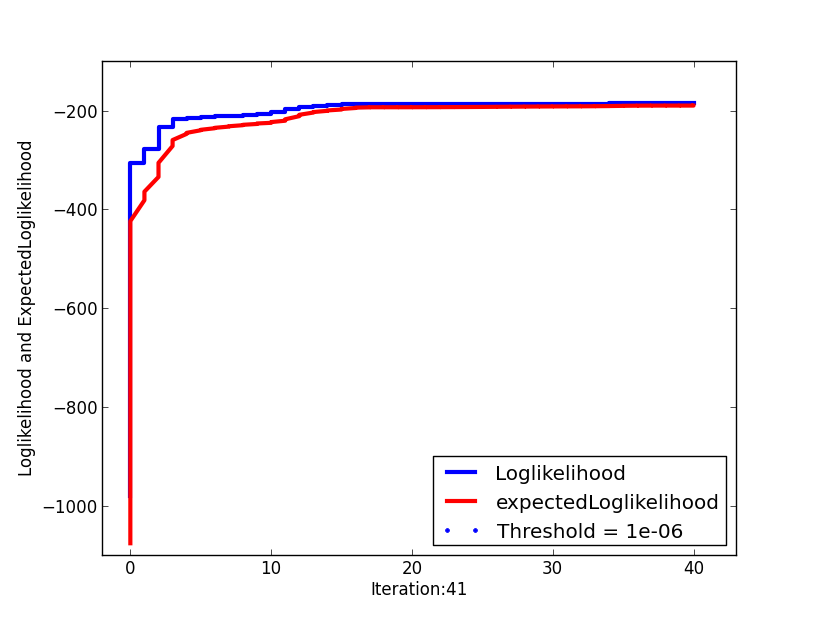
\includegraphics[width=5in,height=3.3in]{./Result/figure_1.png}
\end{center}
\htab Initilisation of parameters:
\begin{align} 
    \bs{\mu}_{0} = \begin{pmatrix} 
6.94825182 & 3.43028943 & 5.13165042 & 1.73043353 
 \end{pmatrix}   \\
    \bs{\mu}_{1} = \begin{pmatrix} 
6.03430983 & 2.44263481 & 4.19416609 & 1.34434648 
 \end{pmatrix}    \\
    \bs{\mu}_{2} = \begin{pmatrix} 
7.41659032 & 2.74307646 & 3.54490011 & 0.37515563 
    \end{pmatrix}  \end{align} \vspace{-1cm}
\begin{align} 
    \bs{\Sigma}_{0} = \bs{\Sigma}_{1} = \bs{\Sigma}_{2} = \bs{I}
\end{align} \vspace{-1cm}
\begin{align}  \bs{\pi} = \begin{pmatrix}
    0.63777939 & 0.17825037 & 0.18397024
\end{pmatrix} \end{align}
\htab Iteration Quantity: 41 \\
\htab Parameters of resulted Guassians:
\begin{align} \bs{\mu}_{0} = \begin{pmatrix} 
6.30229683 & 2.90022864 & 5.06049687 & 1.76245416 
 \end{pmatrix}  \end{align}\vspace{-1cm} 
\begin{align} \bs{\Sigma}_{0}\begin{pmatrix} 
0.42223868 & 0.09703482 & 0.43821003 & 0.15608046 \\ 
0.09703482 & 0.10551541 & 0.11569370 & 0.07015344 \\ 
0.43821003 & 0.11569370 & 0.62024483 & 0.24770913 \\ 
0.15608046 & 0.07015344 & 0.24770913 & 0.16391035 \\ 
\end{pmatrix} \end{align}

\begin{align} \bs{\mu}_{1} = \begin{pmatrix} 
6.06077537 & 2.73103951 & 4.13451491 & 1.24428925 
 \end{pmatrix}  \end{align}\vspace{-1cm} 
\begin{align} \bs{\Sigma}_{1}\begin{pmatrix} 
0.44986364 & 0.20624275 & 0.31552694 & 0.10820035 \\ 
0.20624275 & 0.10624364 & 0.13904845 & 0.05150205 \\ 
0.31552694 & 0.13904845 & 0.23264190 & 0.07652083 \\ 
0.10820035 & 0.05150205 & 0.07652083 & 0.02840178 \\ 
\end{pmatrix} \end{align}

\begin{align} \bs{\mu}_{2} = \begin{pmatrix} 
5.00600023 & 3.42800051 & 1.46200007 & 0.24599998 
 \end{pmatrix}  \end{align}\vspace{-1cm} 
\begin{align} \bs{\Sigma}_{2}\begin{pmatrix} 
0.12176394 & 0.09723179 & 0.01602797 & 0.01012402 \\ 
0.09723179 & 0.14081549 & 0.01146392 & 0.00911203 \\ 
0.01602797 & 0.01146392 & 0.02955600 & 0.00594801 \\ 
0.01012402 & 0.00911203 & 0.00594801 & 0.01088400 \\ 
\end{pmatrix} \end{align}
\begin{align}  \bs{\pi} = \begin{pmatrix}
    0.55543518 & 0.11123164 & 0.33333318
\end{pmatrix} \end{align}
%}}}
\newpage
%{{{ second case
\begin{center}
    \textbf{Specific data in second random initialisation}
    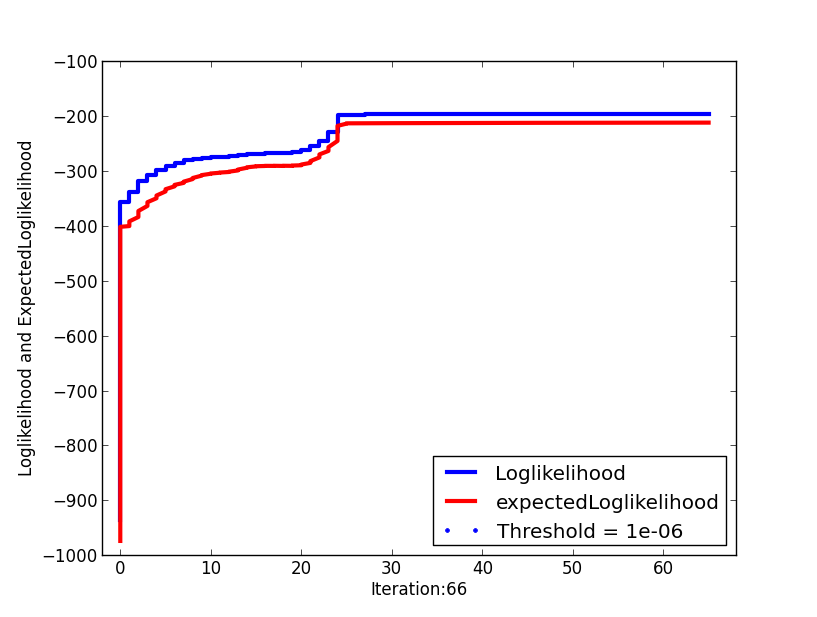
\includegraphics[width=5in,height=3.3in]{./Result/figure_2.png}
\end{center}
\htab Initilisation of parameters:
\begin{align} 
    \bs{\mu}_{0} = \begin{pmatrix} 
        5.47252304 & 3.04349496 & 3.20982127 & 1.74800758 
    \end{pmatrix}   \\
    \bs{\mu}_{1} = \begin{pmatrix} 
        5.37077336 & 3.19556116 & 5.46395648 & -0.03621684 
    \end{pmatrix}    \\
    \bs{\mu}_{2} = \begin{pmatrix} 
        6.08856967 & 3.14829166 & 5.74406265 & 1.40878059
    \end{pmatrix}  \end{align} \vspace{-1cm}
    \begin{align} 
        \bs{\Sigma}_{0} = \bs{\Sigma}_{1} = \bs{\Sigma}_{2} = \bs{I}
    \end{align} \vspace{-1cm}
    \begin{align}  \bs{\pi} = \begin{pmatrix}
        0.92942981 & 0.06546349 & 0.0051067
    \end{pmatrix} \end{align}
\htab Iteration Quantity: 66 \\
\htab Parameters of resulted Guassians:
    \begin{align} \bs{\mu}_{0} = \begin{pmatrix} 
        5.00600011 & 3.42800025 & 1.46200004 & 0.24599999 
    \end{pmatrix}  \end{align}\vspace{-1cm} 
    \begin{align} \bs{\Sigma}_{0}\begin{pmatrix} 
        0.12176397 & 0.09723189 & 0.01602799 & 0.01012401 \\ 
        0.09723189 & 0.14081575 & 0.01146396 & 0.00911202 \\ 
        0.01602799 & 0.01146396 & 0.02955600 & 0.00594800 \\ 
        0.01012401 & 0.00911202 & 0.00594800 & 0.01088400 \\ 
    \end{pmatrix} \end{align}

    \begin{align} \bs{\mu}_{1} = \begin{pmatrix} 
        6.11764829 & 2.84264967 & 4.67930452 & 1.59705880 
    \end{pmatrix}  \end{align}\vspace{-1cm} 
    \begin{align} \bs{\Sigma}_{1}\begin{pmatrix} 
        0.31117193 & 0.10177389 & 0.28584863 & 0.14245983 \\ 
        0.10177389 & 0.09664535 & 0.12171721 & 0.07841352 \\ 
        0.28584863 & 0.12171721 & 0.47102262 & 0.24838159 \\ 
        0.14245983 & 0.07841352 & 0.24838159 & 0.17198206 \\ 
    \end{pmatrix} \end{align}

    \begin{align} \bs{\mu}_{2} = \begin{pmatrix} 
        6.90609957 & 3.00296152 & 5.91751825 & 2.02823662 
    \end{pmatrix}  \end{align}\vspace{-1cm} 
    \begin{align} \bs{\Sigma}_{2}\begin{pmatrix} 
        0.47944373 & 0.10318151 & 0.37851617 & -0.00947992 \\ 
        0.10318151 & 0.14649679 & 0.06689303 & 0.02639494 \\ 
        0.37851617 & 0.06689303 & 0.33139405 & 0.01686062 \\ 
        -0.00947992 & 0.02639494 & 0.01686062 & 0.05638487 \\ 
    \end{pmatrix} \end{align}
    \begin{align}  \bs{\pi} = \begin{pmatrix}
        0.33333326 & 0.54461183 & 0.12205491
    \end{pmatrix} \end{align}
    %}}}
\newpage
    %{{{ third case
    \begin{center}
        \textbf{Specific data in third random initialisation}
        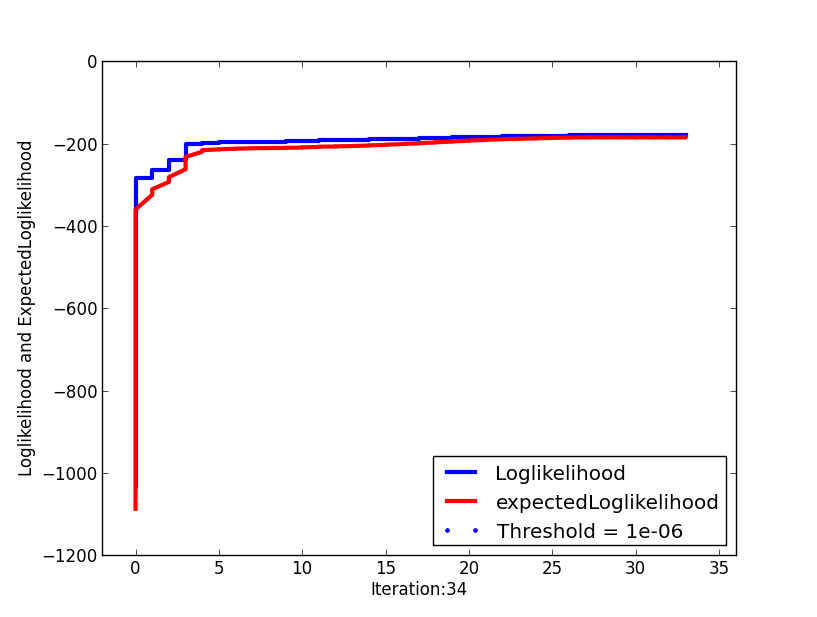
\includegraphics[width=5in,height=3.3in]{./Result/figure_3.png}
    \end{center}
    \htab Initilisation of parameters:
    \begin{align} 
        \bs{\mu}_{0} = \begin{pmatrix} 
            5.58180881 & 4.84821904 & 4.19996763 & 1.66923484 
        \end{pmatrix}   \\
        \bs{\mu}_{1} = \begin{pmatrix} 
            5.98138886 & 3.26599148 & 2.48486145 & -0.38105446 
        \end{pmatrix}    \\
        \bs{\mu}_{2} = \begin{pmatrix} 
            5.81470396 & 4.52844168 & 4.91642107 & 3.99937301 
        \end{pmatrix}  \end{align} \vspace{-1cm}
        \begin{align} 
            \bs{\Sigma}_{0} = \bs{\Sigma}_{1} = \bs{\Sigma}_{2} = \bs{I}
        \end{align} \vspace{-1cm}
        \begin{align}  \bs{\pi} = \begin{pmatrix}
            0.5694223 & 0.22911455 & 0.20146316
        \end{pmatrix} \end{align}
        \htab Iteration Quantity: 34 \\
        \htab Parameters of resulted Guassians:
        \begin{align} \bs{\mu}_{0} = \begin{pmatrix} 
            5.91506499 & 2.77785242 & 4.20175063 & 1.29704350 
        \end{pmatrix}  \end{align}\vspace{-1cm} 
        \begin{align} \bs{\Sigma}_{0}\begin{pmatrix} 
            0.27532206 & 0.09691983 & 0.18469154 & 0.05440596 \\ 
            0.09691983 & 0.09264056 & 0.09113461 & 0.04299639 \\ 
            0.18469154 & 0.09113461 & 0.20070652 & 0.06101118 \\ 
            0.05440596 & 0.04299639 & 0.06101118 & 0.03201270 \\ 
        \end{pmatrix} \end{align}

        \begin{align} \bs{\mu}_{1} = \begin{pmatrix} 
            5.00600000 & 3.42800000 & 1.46200000 & 0.24600000 
        \end{pmatrix}  \end{align}\vspace{-1cm} 
        \begin{align} \bs{\Sigma}_{1}\begin{pmatrix} 
            0.12176400 & 0.09723200 & 0.01602800 & 0.01012400 \\ 
            0.09723200 & 0.14081600 & 0.01146400 & 0.00911200 \\ 
            0.01602800 & 0.01146400 & 0.02955600 & 0.00594800 \\ 
            0.01012400 & 0.00911200 & 0.00594800 & 0.01088400 \\ 
        \end{pmatrix} \end{align}

        \begin{align} \bs{\mu}_{2} = \begin{pmatrix} 
            6.54467220 & 2.94870862 & 5.47980119 & 1.98476235 
        \end{pmatrix}  \end{align}\vspace{-1cm} 
        \begin{align} \bs{\Sigma}_{2}\begin{pmatrix} 
            0.38704847 & 0.09220736 & 0.30276907 & 0.06159530 \\ 
            0.09220736 & 0.11034094 & 0.08425917 & 0.05599446 \\ 
            0.30276907 & 0.08425917 & 0.32766484 & 0.07441712 \\ 
            0.06159530 & 0.05599446 & 0.07441712 & 0.08573678 \\ 
        \end{pmatrix} \end{align}
        \begin{align}  \bs{\pi} = \begin{pmatrix}
            0.29931064 & 0.33333333 & 0.36735603
        \end{pmatrix} \end{align}
        %}}}
\newpage
%{{{ fourth case
\begin{center}
    \textbf{Specific data in fourth random initialisation}
    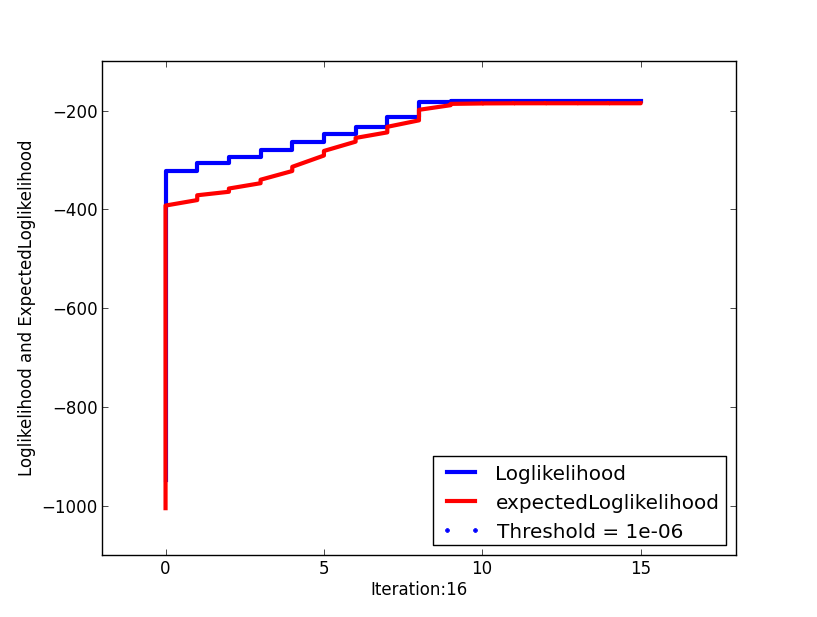
\includegraphics[width=5in,height=3.3in]{./Result/figure_4.png}
\end{center}
\htab Initilisation of parameters:
\begin{align} 
    \bs{\mu}_{0} = \begin{pmatrix} 
4.93395858 & 3.72289358 & 2.88809351 & 1.81106115
 \end{pmatrix}   \\
    \bs{\mu}_{1} = \begin{pmatrix} 
5.74870051 & 1.17972676 & 3.84560644 & 0.78416837 
 \end{pmatrix}    \\
    \bs{\mu}_{2} = \begin{pmatrix} 
7.63689574 & 2.95945543 & 5.19796747 & 1.71749004
    \end{pmatrix}  \end{align} \vspace{-1cm}
\begin{align} 
    \bs{\Sigma}_{0} = \bs{\Sigma}_{1} = \bs{\Sigma}_{2} = \bs{I}
\end{align} \vspace{-1cm}
\begin{align}  \bs{\pi} = \begin{pmatrix}
    0.86693085 & 0.06884158 & 0.06422758
\end{pmatrix} \end{align}
\htab Iteration Quantity: 16 \\
\htab Parameters of resulted Guassians:
\begin{align} \bs{\mu}_{0} = \begin{pmatrix} 
5.00600000 & 3.42800000 & 1.46200000 & 0.24600000 
 \end{pmatrix}  \end{align}\vspace{-1cm} 
\begin{align} \bs{\Sigma}_{0}\begin{pmatrix} 
0.12176400 & 0.09723200 & 0.01602800 & 0.01012400 \\ 
0.09723200 & 0.14081600 & 0.01146400 & 0.00911200 \\ 
0.01602800 & 0.01146400 & 0.02955600 & 0.00594800 \\ 
0.01012400 & 0.00911200 & 0.00594800 & 0.01088400 \\ 
\end{pmatrix} \end{align}

\begin{align} \bs{\mu}_{1} = \begin{pmatrix} 
5.91510204 & 2.77785066 & 4.20180128 & 1.29706329 
 \end{pmatrix}  \end{align}\vspace{-1cm} 
\begin{align} \bs{\Sigma}_{1}\begin{pmatrix} 
0.27532744 & 0.09691654 & 0.18470680 & 0.05441350 \\ 
0.09691654 & 0.09264040 & 0.09113279 & 0.04299613 \\ 
0.18470680 & 0.09113279 & 0.20073024 & 0.06102147 \\ 
0.05441350 & 0.04299613 & 0.06102147 & 0.03201724 \\ 
\end{pmatrix} \end{align}

\begin{align} \bs{\mu}_{2} = \begin{pmatrix} 
6.54468870 & 2.94872272 & 5.47985468 & 1.98479721 
 \end{pmatrix}  \end{align}\vspace{-1cm} 
\begin{align} \bs{\Sigma}_{2}\begin{pmatrix} 
0.38706100 & 0.09220597 & 0.30277029 & 0.06158850 \\ 
0.09220597 & 0.11033973 & 0.08424916 & 0.05598870 \\ 
0.30277029 & 0.08424916 & 0.32763930 & 0.07439355 \\ 
0.06158850 & 0.05598870 & 0.07439355 & 0.08572418 \\ 
\end{pmatrix} \end{align}
\begin{align}  \bs{\pi} = \begin{pmatrix}
    0.33333333 & 0.29933787  & 0.36732879
\end{pmatrix} \end{align}
%}}}
\newpage
%{{{ fifth case
\begin{center}
    \textbf{Specific data in fifth random initialisation}
    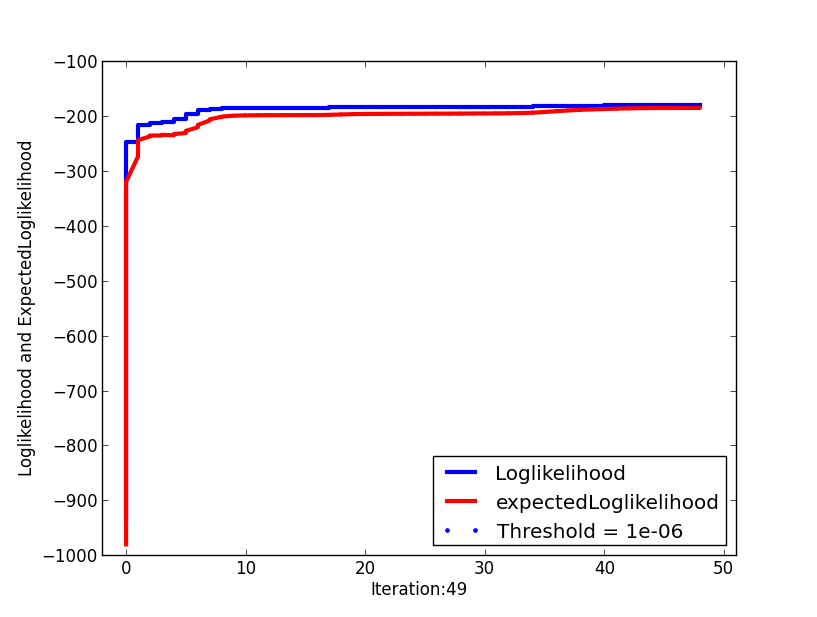
\includegraphics[width=5in,height=3.3in]{./Result/figure_5.png}
\end{center}
\htab Initilisation of parameters:
\begin{align} 
    \bs{\mu}_{0} = \begin{pmatrix} 
4.74122040 & 3.15279417 & 1.77909908 & 0.80293032 
 \end{pmatrix}   \\
    \bs{\mu}_{1} = \begin{pmatrix} 
6.36558270 & 4.20423977 & 4.12724521 & 1.24996769 
 \end{pmatrix}    \\
    \bs{\mu}_{2} = \begin{pmatrix} 
7.34388669 & 3.54991993 & 4.39371314 & 2.05949636 
    \end{pmatrix}  \end{align} \vspace{-1cm}
\begin{align} 
    \bs{\Sigma}_{0} = \bs{\Sigma}_{1} = \bs{\Sigma}_{2} = \bs{I}
\end{align} \vspace{-1cm}
\begin{align}  \bs{\pi} = \begin{pmatrix}
    0.02053414 & 0.0965958 &  0.88287006
\end{pmatrix} \end{align}
\htab Iteration Quantity: 49 \\
\htab Parameters of resulted Guassians:
\begin{align} \bs{\mu}_{0} = \begin{pmatrix} 
5.00600000 & 3.42800000 & 1.46200000 & 0.24600000 
 \end{pmatrix}  \end{align} \vspace{-1cm} 
\begin{align} \bs{\Sigma}_{0}\begin{pmatrix} 
0.12176400 & 0.09723200 & 0.01602800 & 0.01012400 \\ 
0.09723200 & 0.14081600 & 0.01146400 & 0.00911200 \\ 
0.01602800 & 0.01146400 & 0.02955600 & 0.00594800 \\ 
0.01012400 & 0.00911200 & 0.00594800 & 0.01088400 \\ 
\end{pmatrix} \end{align}

\begin{align} \bs{\mu}_{1} = \begin{pmatrix} 
5.91484076 & 2.77783583 & 4.20129188 & 1.29686598 
 \end{pmatrix}  \end{align} \vspace{-1cm} 
\begin{align} \bs{\Sigma}_{1}\begin{pmatrix} 
0.27531479 & 0.09697069 & 0.18462390 & 0.05437052 \\ 
0.09697069 & 0.09265277 & 0.09115580 & 0.04299921 \\ 
0.18462390 & 0.09115580 & 0.20053150 & 0.06093600 \\ 
0.05437052 & 0.04299921 & 0.06093600 & 0.03197655 \\ 
\end{pmatrix} \end{align}

\begin{align} \bs{\mu}_{2} = \begin{pmatrix} 
6.54438345 & 2.94859425 & 5.47921795 & 1.98439211 
 \end{pmatrix}  \end{align} \vspace{-1cm} 
\begin{align} \bs{\Sigma}_{2}\begin{pmatrix} 
0.38703762 & 0.09221031 & 0.30286958 & 0.06172628 \\ 
0.09221031 & 0.11033498 & 0.08432941 & 0.05603638 \\ 
0.30286958 & 0.08432941 & 0.32798018 & 0.07468452 \\ 
0.06172628 & 0.05603638 & 0.07468452 & 0.08588114 \\ 
\end{pmatrix} \end{align}
\begin{align}  \bs{\pi} = \begin{pmatrix}
     0.33333333 & 0.29903553 & 0.36763114
\end{pmatrix} \end{align}

\newpage
%}}}
\end{document}

% above a useless things
%{{{
\htab Based on the probability distribution of measurement $\x$ conditioned on $z_{k}$, 
    \begin{align}
        p(\x | z_{k} = 1) 
        &= \N(\bmu_{k} | \sigma^{2} \bs{I})
    \end{align}
\htab Since we use 1-of-k coding scheme, at all states of $\z$, only one element $z_{k}$ can be one while
others are zeros. That is, no measurement is from two trees, which conforms to our assumption in the question
that the trees have a small diameter and thus the offset of measurement from the true center is negligible.
Therefore, we can repreent $p(\x | \z)$ in the way as follows,
\begin{align}
    p(\x | \z) &= \prodk \Big( \Nx \Big)^{z_{k}} \label{7:x|zk}
    \end{align}
\htab Similarly according to the 1-of-k coding scheme, set the $p(z_{k} = 1) = \pk$,
in order to derive $p(\z)$, we have
    \begin{align}
        p(\z) = \prodk \pk^{z_{k}} \label{7:pz}
    \end{align}
\htab Consider the distribution of laser-range measurement $p(\x, \z)$
    \begin{align}
        p(\x, \z) 
        &= \ p(\z)\ p(\x | \z)  &&\mbox{product rule} \\
        &=  \prodk \pk^{z_{k}} \prodk \Nx ^{z_{k}} 
        &&\mbox{cite \eqref{7:x|zk} and \eqref{7:pz}} \\
        &= \prodk \Big(  \pk  \Nx  \Big)^{z_{k}}
        &&\mbox{abstract the multiplication}
    \end{align}
\htab Again, based on the 1-of-k coding scheme, for each measurement $\x_{n}$, the corresponding latent
    variable has only one element $z_{k}=1$ and others $z_{k}=0$. If we use $k$ to denote always the non-zero 
    element index of $\z$, we can ignore the
    multiplication over $k$ towards the terms with power of $z_{k}$ and derive the following
    representation of $p(\x, \z)$.
\begin{align}
    p(\x, \z) 
     &= \pk \N(\bmu_{k} | \sigma^{2} \bs{I})  \\
     &=  \pk \Nx  \label{7:jointprob}
    \end{align}
\htab Based on the sum rule, we derive the objective,
\begin{align}
    p(\x) = \sumz p(\x, \z)
    &= \sumz \pk \N(\bmu_{k} | \sigma^{2} \bs{I})  \\
     &=  \sumk \pk \Nx  \label{7:univariateprob}
    \end{align}
\htab The explanation to the last step of above derivation is that summing over all states of $z$ is to
sum over all possible $k$ for which $z_{k} = 1$ under the condition of 1-of-k coding scheme. \\
\htab Then seek to figure out the likelihood of collecting a series of data objects,
    \begin{align}
        L(\XX) 
        &= \prod_{n=1}^{N} p(\xn)  &&\mbox{i.i.d} \\
        &= \prodn \sumk \pk \Nk  
        &&\mbox{cite \eqref{7:univariateprob}} \label{6:liki}
    \end{align}
\htab Then take the logarithm to the likelihood of observations \eqref{6:liki},
    \begin{align}
        ln (L(\XX)) 
        &=  \sum_{n=1}^{N} ln \Big( \sum_{k=1}^{K} \pi_{k}\ \Nk \Big)
        \label{7:logliki}
    \end{align} 
\htab where the $\N(\bmu_{k} | \sigma^{2} \bs{I})$ is gaussian distribution of the form as follows,
\begin{align}
    \Nk = \frac{1}{(2\pi)^{\frac{D}{2}} \sigma^{D}} exp \Big( -\frac{(\difxm)^{T} (\difxm)}{2\sigma^{2}}\Big)
    \end{align}
%}}}
%}}}

